\documentclass[lang=cn,10pt]{elegantbook}

\title{东邪的机器学习之旅}


\author{dx}

\date{2025，8，19}
\version{1.0}
\bioinfo{自定义}{信息}

\extrainfo{不要以为抹消过去，重新来过，即可发生什么改变。—— 比企谷八幡}

\setcounter{tocdepth}{3}

\logo{logo-blue.png}
\cover{cover.jpg}

% 本文档命令
\usepackage{array}
\newcommand{\ccr}[1]{\makecell{{\color{#1}\rule{1cm}{1cm}}}}

% 修改标题页的橙色带
% \definecolor{customcolor}{RGB}{32,178,170}
% \colorlet{coverlinecolor}{customcolor}

\begin{document}

\maketitle
\frontmatter

\tableofcontents

\mainmatter
\chapter{PCA}
\begin{definition}[Principal Component Analysis]
主成分分析（PCA）是一种无监督学习算法，用于降维并识别数据中最具信息量的特征。

它的本质思想是：假设数据关系具有线性结构，并将其投影到一个由正交向量组成的子空间中，使得方差最大化。这样的向量称为主成分，它们决定了数据变化最大（信息量最高）的方向。

另一种等价的理解是：PCA 可以看作一种线性投影，它最小化了原始点与其投影点之间的均方根（RMS）距离。

\end{definition}

PCA 的工作原理

首先，特征矩阵需要进行中心化处理，以确保第一主成分对应的是数据的最大变化方向，而不仅仅是平均值。通常，求主成分的方法有两种主要思路：
第一，协方差矩阵的特征值与特征向量分解。协方差矩阵反映了不同变量之间的线性相关程度。该矩阵的特征向量给出了数据方差最大的方向，而特征值则表示该方向上的方差大小。与某个特征向量对应的特征值刻画了该向量对解释数据方差的贡献。特征值越大，该主成分的重要性就越高。通常，只选择能够解释预设方差比例（如 95\%）的主成分。
\section{协方差矩阵理解}
\begin{definition}[3.3.1]
设 $(X_1, X_2, \ldots, X_n)$ 是 $n$ 维随机变量，若 $E(X_1), E(X_2), \ldots, E(X_n)$ 存在，则称 
\[
(E(X_1), E(X_2), \ldots, E(X_n))
\]
为 $(X_1, X_2, \ldots, X_n)$ 的数学期望，简称期望。  

\medskip
固定 $i,j$，若 
\[
E\bigl([X_i - E(X_i)][X_j - E(X_j)]\bigr)
\]
存在，则称其为 $X_i$ 与 $X_j$ 的协方差（covariance），记作 $\mathrm{Cov}(X_i, X_j)$，即
\[
\mathrm{Cov}(X_i, X_j) = E\bigl([X_i - E(X_i)][X_j - E(X_j)]\bigr).
\]

\medskip
易知，$E(X_i)$ 和 $E(X_j)$ 存在是 $\mathrm{Cov}(X_i, X_j)$ 存在的必要条件。  

\medskip
若对 $i,j = 1,2,\ldots,n$，所有 $\mathrm{Cov}(X_i, X_j)$ 均存在，则称 $n$ 阶方阵
\[
\Sigma = (b_{ij})_{n\times n}, \quad b_{ij} = \mathrm{Cov}(X_i, X_j)
\]
为 $(X_1, X_2, \ldots, X_n)$ 的协方差矩阵（covariance matrix）。
\end{definition}


\begin{dxtips}{方差与协方差总结}[PS]\label{dx:any-construct}


\textbf{1. 定义}  
\[
\mathrm{Var}(X) = E\big[(X - E[X])^2\big], \qquad
\mathrm{Cov}(X,Y) = E\big[(X - E[X])(Y - E[Y])\big]
\]

\medskip
\textbf{2. 数学关系}  
\[
\mathrm{Var}(X) = \mathrm{Cov}(X,X)
\]
方差是协方差的特例。

\medskip
\textbf{3. 性质比较}  

\begin{tabular}{|c|c|c|}
\hline
性质 & 方差 Var(X) & 协方差 Cov(X,Y) \\\hline
定义 & 单变量的离散程度 & 两变量的联动程度 \\\hline
符号 & $\ge 0$ & 可正、可负、或为 0 \\\hline
几何意义 & 数据点围绕均值的分布宽度 & 点云的倾斜方向、线性关系 \\\hline
特殊情况 & $\mathrm{Var}(X)=0 \iff X$ 为常数 & $\mathrm{Cov}(X,Y)=0 \not\Rightarrow$ 独立 \\\hline
\end{tabular}


\end{dxtips}

里面的$ E(\cdot)$ 就是 期望算子，它的作用就是“取加权平均”。
情景：两门考试成绩。设三名学生的语文与数学成绩分别为
A：$X=50,\,Y=55$，B：$X=60,\,Y=65$，C：$X=70,\,Y=75$。

\begin{enumerate}
  \item 算平均值（期望）：
  \[
    E[X]=\frac{50+60+70}{3}=60,\qquad
    E[Y]=\frac{55+65+75}{3}=65.
  \]
  \item 偏离均值：
  \[
  \begin{aligned}
    &\text{A: }X-60=-10,\; Y-65=-10;\\
    &\text{B: }X-60=0,\;   Y-65=0;\\
    &\text{C: }X-60=10,\;  Y-65=10.
  \end{aligned}
  \]
  \item 偏离乘积：
  \[
    \text{A: }(-10)(-10)=100,\qquad
    \text{B: }0\cdot 0=0,\qquad
    \text{C: }10\cdot 10=100.
  \]
  \item 取平均（期望）得到协方差：
  \[
    \mathrm{Cov}(X,Y)
    =E\!\big[(X-E[X])(Y-E[Y])\big]
    =\frac{100+0+100}{3}
    =\frac{200}{3}\approx 66.7.
  \]
\end{enumerate}

结果解读：协方差为正，说明语文高的一般数学也高（正相关）；若为负则一高一低（负相关）；若接近 $0$，则两者几乎无线性关系。
协方差矩阵就是把所有不同的Xi和Xy的关联性在一个矩阵中记录出来。
\begin{dxtips}
    进一步来说来说减法是把所有的x轴上的点左移或者右移，Y轴的点上移或者下移，两个合起来的操作就是把坐标系切换成了以他们均值为原点的坐标系。他们的乘积就是每一个坐标和原点围成矩形的面积，加权的方式可以让你觉得哪一部分的重要凸显，比如说我希望进缩小极大偏离平均值的那项对整体的影响我就可以给他加一个小的权重让他生成的矩阵面积缩小。
 \\
	•	协方差不仅是“面积”，还是一种 趋势的代数平均。
	•	如果绝大多数点落在“同向象限”（右上、左下），那么平均面积大于 0 → 正相关。
	•	如果大多数点落在“反向象限”（右下、左上），平均面积小于 0 → 负相关。
	•	如果点云分布比较均匀，正负面积互相抵消 → 协方差接近 0。
\end{dxtips}
协方差的几何意义有助于理解其方向与强度，可参见下列视频：\url{https://www.bilibili.com/video/BV1UWYfz2EKZ}









\section{SVD奇异值分解}


第二，数据矩阵的奇异值分解 (SVD)。奇异值分解将任意矩阵表示为三个矩阵的乘积：左奇异矩阵 $U$、奇异值对角矩阵 $S$、以及右奇异矩阵 $V$。其中，奇异值是协方差矩阵特征值的平方根（这就是为什么需要先对数据做中心化），右奇异矩阵 $V$ 对应于协方差矩阵的特征向量，而左奇异矩阵 $U$ 则是原始数据在主成分上的投影。因此，SVD 也可以提取出主成分，而且无需显式计算协方差矩阵。与特征分解方法相比，这种方式更高效、更数值稳定，尤其是在特征间存在强相关性、导致协方差矩阵条件数较差的情况下。特别地，scikit-learn 的 PCA 实现采用的就是这种方法，不过还结合了一些额外的技巧。
\begin{dxtips}{特征值与奇异值}
    

奇异值与特征值在定义和几何意义上既有联系又有区别。对于方阵 $A \in \mathbb{R}^{n\times n}$，若存在 $\lambda$ 使得 $Av=\lambda v$（$v\neq 0$），则 $\lambda$ 称为 $A$ 的特征值；而对于任意矩阵 $A \in \mathbb{R}^{m\times n}$，若存在 $\sigma$ 使得 $A^{\mathsf T} A v=\sigma^2 v$（$v\neq 0$），则 $\sigma$ 称为 $A$ 的奇异值，即奇异值是 $A^{\mathsf T}A$ 的特征值的非负平方根。因此奇异值永远非负，而特征值可能为正或负。进一步地，如果 $A$ 是对称矩阵，则奇异值等于特征值的绝对值。例如 $A=\begin{bmatrix}-3&0\\0&2\end{bmatrix}$ 的特征值为 $-3,2$，而奇异值为 $3,2$。\\在几何意义上，特征值描述了矩阵在某些特定方向上对向量的缩放因子，而奇异值则表示矩阵将单位球拉伸为椭球时的半轴长度，刻画的是整体的伸缩尺度。换句话说，奇异值等于 $A^{\mathsf T}A$ 的特征值平方根，而在对称矩阵的情形下，奇异值就是特征值的绝对值。
\end{dxtips}
\subsection{为什么要把矩阵转化为向量乘积}

一个 $m\times n$ 的矩阵一共有 $mn$ 个单元，但是一列加一行只有 $m+n$ 个分量。  
为了快速处理矩阵，往往需要将其转化为分量乘积的形式。简单来说，一个图像可以视为一个大型矩阵。  
要完美复制它，我们需要 $8mn$ 比特的信息。  

高分辨率电视通常有 $m=1080$ 与 $n=1920$，每秒通常有 $24$ 帧，而且你可能喜欢看彩色画面（$3$ 个颜色通道）。  
因此总共需要传输
\[
3 \times 8 \times (1080 \times 1920 \times 24) \;=\; 3\times 8 \times 48,470,400
\]
比特每秒。  
这太昂贵而且不可行，传输器也跟不上表演的速度。  

当压缩做得很好时，你几乎看不出与原始图像的差别。图像的边缘（即灰度的突然改变）是最难压缩的部分。  
如果每个 $a_{ij}$ 都是无关的随机数字，那么压缩根本不可能成功。我们完全依赖这样的事实：邻近像素通常具有相似的灰度值。  
当你跨越边缘时，会产生一个突跳。现实世界的图像中边缘无处不在，所以动画相比静止图像更容易压缩。\\
\subsection{为什么还需要SVD分解}
Singular Value Decomposition，
\begin{example}[2]
``“王牌旗'' 法国国旗 $A$，意大利国旗 $A$，德国国旗 $A^{\mathsf T}$

\[
A =
\begin{bmatrix}
a & a & c & c & e & e\\
a & a & c & c & e & e\\
a & a & c & c & e & e\\
a & a & c & c & e & e\\
a & a & c & c & e & e\\
a & a & c & c & e & e
\end{bmatrix}
\quad\longrightarrow\quad
\begin{bmatrix}
1\\1\\1\\1\\1\\1
\end{bmatrix}
\begin{bmatrix}
a & a & c & c & e & e
\end{bmatrix}
\]

国旗有 3 个颜色但是秩还是 $1$。假设这 36 个单元保持秩 $1$ 的模式 $A = u_1 v_1^{\mathsf T}$，它们甚至可以全部不相同。
但是当秩变成 $r=2$ 时，我们需要 $u_1 v_1^{\mathsf T} + u_2 v_2^{\mathsf T}$。\textcolor{red}{秩是几就需要几个不线性相关的矩阵，每个矩阵都可以写成行乘列}
\end{example}

\begin{example}[3 嵌入方形]
\[
A=
\begin{bmatrix}
1 & 0\\
1 & 1
\end{bmatrix}
\quad=\quad
\begin{bmatrix}
1\\1
\end{bmatrix}
\begin{bmatrix}
1 & 1
\end{bmatrix}
-
\begin{bmatrix}
1\\0
\end{bmatrix}
\begin{bmatrix}
0 & 1
\end{bmatrix}.
\]

$A$ 的 $1$ 与 $0$ 可以是 $1$ 的方块与 $0$ 的方块。秩仍然是 $2$，我们仍然只需要两个项 $u_1 v_1^{\mathsf T}+u_2 v_2^{\mathsf T}$。
一个 $6\times 6$ 图像可以由 24 个数字压缩而来；一个 $N\times N$ 图像 ($N^2$ 个数字) 可以压缩成 4 个向量 $u_1,u_2,v_1,v_2$ 的 $4N$ 个数字。

注意：这并不是来自 SVD 的选择！例如 $u_1=(1,1), u_2=(1,0)$ 没有正交；
$u_1=(1,1)$ 与 $v_2=(0,1)$ 也没有正交。SVD 会保证按照顺序选择秩 $1$ 片段。
\end{example}

\begin{dxtips}[正交化的好处]
    

 唯一性：正交基保证分解几乎唯一，不会乱选。
\\ 简洁几何意义：任何矩阵 = 旋转 + 拉伸 + 再旋转。
\\数值稳定：正交基避免冗余，误差不放大。
\\ 最优近似：保留前几个奇异值就得到最小误差的低秩近似。
\end{dxtips}
\subsection{如何寻找正交化基底}
ATA是半正定而且对称的他天然自带一组正交基，AAT同理我们这样就得倒了两组正交基。
\begin{tcolorbox}[colback=blue!5!white, colframe=blue!75!black, title=来自 SVD 的选择]
\[
AA^{\mathsf T} u_i = \sigma_i^2 u_i,
\qquad
A^{\mathsf T} A v_i = \sigma_i^2 v_i,
\qquad
A v_i = \sigma_i u_i
\]
\end{tcolorbox}
\[
AA^{\mathsf T}Av_i=\sigma_i^2 Av_i 
\;\Rightarrow\; 
Av_i \text{ 是 } AA^{\mathsf T} \text{ 的特征向量，对应特征值 } \sigma_i^2.
\]

\[
\text{因此 } Av_i=u_i, \text{ 但此时的 } u_i \text{ 还不是单位向量，需要计算 } Av_i \text{ 的长度：}
\]

\[
\|Av_i\|^2
= (Av_i)^{\mathsf T}(Av_i)
= v_i^{\mathsf T}(A^{\mathsf T}A)v_i
= v_i^{\mathsf T}(\sigma_i^2 v_i)
= \sigma_i^2 \|v_i\|^2
= \sigma_i^2.
\]

\[
\Rightarrow\quad \|Av_i\|=\sigma_i, 
\qquad 
u_i=\tfrac{1}{\sigma_i}Av_i.
\]
\begin{dxtips}
    因为特征向量乘一个系数还是特征向量所以要看清到底指的那个，比如这里要求的就是单位化的。单位化的一大好处就是满秩正交矩阵乘自己的转置等于单位矩阵可以消除项。
\end{dxtips}

由 $Av_i=\sigma_i u_i$ 可得
\[
A v_i v_i^{\mathsf T}=(A v_i)\,v_i^{\mathsf T}=\sigma_i u_i v_i^{\mathsf T},
\]
它表示 $A$ 在第 $i$ 个方向上的秩一部分：该矩阵将任意输入向量在 $v_i$ 方向上的分量提取出来，并映射到 $u_i$ 方向上，因而秩为 $1$（若 $\sigma_i=0$ 则为 $0$）。
\\整体的式子如下
\[
A V V^{\mathsf T} \;=\; U \Sigma V^{\mathsf T}, 
\qquad V V^{\mathsf T} = I, 
\qquad \Rightarrow\; A = U \Sigma V^{\mathsf T}.
\]其中 $\Sigma$ 是一个对角矩阵
\[
\Sigma = \mathrm{diag}(\sigma_1, \sigma_2, \dots, \sigma_r).
\]\[
A 
= 
\begin{bmatrix} u_1 & u_2 \end{bmatrix}
\begin{bmatrix} \sigma_1 & 0 \\ 0 & \sigma_2 \end{bmatrix}
\begin{bmatrix} v_1^{\mathsf T} \\ v_2^{\mathsf T} \end{bmatrix}
\quad\text{或更简单的}\quad
A \begin{bmatrix} v_1 & v_2 \end{bmatrix}
= \begin{bmatrix} \sigma_1 u_1 & \sigma_2 u_2 \end{bmatrix}.
\]
\\
$\sigma $矩阵在中间，是因为矩阵运算中是后一个矩阵对前一个矩阵作用产生变换， \\
这里 $\sigma$ 是为了得到 $u$ 的系数（即缩放），所以要放在 $U$ 矩阵的前面。

\subsection{奇异值分解计算方法}
SVD 的 $u$'s 称为左奇异向量（$AA^{\mathsf T}$ 的单位特征向量），
$v$'s 称为右奇异向量（$A^{\mathsf T}A$ 的单位特征向量），
$\sigma$'s 是奇异值，就是 $AA^{\mathsf T}$ 与 $A^{\mathsf T}A$ 的相同特征值的平方根：



在范例 3（嵌入方形）中，下列是对称矩阵 $AA^{\mathsf T}$ 与 $A^{\mathsf T}A$：

\[
AA^{\mathsf T}=
\begin{bmatrix}1&0\\1&1\end{bmatrix}
\begin{bmatrix}1&1\\0&1\end{bmatrix}
=
\begin{bmatrix}1&1\\1&2\end{bmatrix},
\qquad
A^{\mathsf T}A=
\begin{bmatrix}1&1\\0&1\end{bmatrix}
\begin{bmatrix}1&0\\1&1\end{bmatrix}
=
\begin{bmatrix}2&1\\1&1\end{bmatrix}.
\]

它们的行列式是 $1$，所以 $\lambda_1 \lambda_2=1$，迹（对角线的和）是 $3$：

\[
\det\begin{bmatrix}1-\lambda & 1\\1 & 2-\lambda\end{bmatrix}
= \lambda^2-3\lambda+1=0,
\]
得到
\[
\lambda_1 = \tfrac{3+\sqrt{5}}{2}, \qquad
\lambda_2 = \tfrac{3-\sqrt{5}}{2}.
\]

$\lambda_1,\lambda_2$ 的平方根是
\[
\sigma_1=\tfrac{\sqrt{5}+1}{2}, \qquad
\sigma_2=\tfrac{\sqrt{5}-1}{2},
\]
且 $\sigma_1\sigma_2=1$。

---

最接近 $A$ 的秩 1 矩阵是 $\sigma_1 u_1 v_1^{\mathsf T}$，误差只有 $\sigma_2\approx 0.6$，是最佳可能。

$AA^{\mathsf T}$ 与 $A^{\mathsf T}A$ 的正交单位特征向量是：
\[
u_1=\begin{bmatrix}1\\ \sigma_1\end{bmatrix}, \quad
u_2=\begin{bmatrix}\sigma_1\\ -1\end{bmatrix}, \quad
v_1=\begin{bmatrix}1\\1\end{bmatrix}, \quad
v_2=\begin{bmatrix}1\\ -\sigma_1\end{bmatrix},
\]
全部除以 $\sqrt{1+\sigma_1^2}$。
\\像通常有满秩，但是他们确实
有低效率的(low effective)秩，这就表示：很多奇异值很小，可以被设定成零。我
们传输的是低秩的近似
压缩时我们丢弃小的$\sigma$ 不会严重损失图像的品质，

\begin{dxtips}[对角化的好处]
    
\begin{enumerate}
  \item 运算简化：$A^k = P D^k P^{-1}$，复杂矩阵运算化为标量运算。
  \item 结构清晰：在特征向量基下，矩阵只表现为伸缩（按特征值缩放）。
  \item 理论方便：如解微分方程、研究马尔可夫链，化为一维问题。
  \item 易于分析：长期行为由最大特征值主导，可用于近似与压缩。
\end{enumerate}
\end{dxtips}
奇异值分解是线性代数的一个亮点，A 的任意 mn 矩阵，方形或矩形，它的
秩是 r。我们会对角化 A，但不是用 X
1
AX，X 里面的特征向量有三个大问题：他
们通常不是正交，不一定有足够的特征向量，而且 Ax = x 要求 A 是方形。A 的
奇异向量以完美的方式解决了全部的问题。
\subsection{奇异值分解也可以满足不满秩的情况}
（使用向量 $u$’s 与 $v$’s 产生 4 个基础子空间的基底：）

\[
\begin{array}{ll}
u_1, \ldots, u_r & \text{是列空间的一组正交单位基底} \\
u_{r+1}, \ldots, u_m & \text{是左零空间 } N(A^{\mathsf T}) \text{ 的一组正交单位基底} \\
v_1, \ldots, v_r & \text{是行空间的一组正交单位基底} \\
v_{r+1}, \ldots, v_n & \text{是零空间 } N(A) \text{ 的一组正交单位基底}
\end{array}
\]
这些 $v$’s 与 $u$’s 负责 $A$ 的行空间与列空间，  
我们还有 $n-r$ 个 $v$’s 与 $m-r$ 个 $u$’s，分别来自零空间 $N(A)$ 与左零空间 $N(A^{\mathsf T})$。  
他们自动与前面 $v$’s 与 $u$’s 正交（因为整个零空间是正交）。  
我们现在引入 $V$ 与 $U$ 的所有 $v$’s 与 $u$’s，所以矩阵变成方形，我们仍然有 $AV = U\Sigma$。

\[
(m \times n)(n \times n) \quad AV = U \Sigma \quad (m \times m)(m \times n)
\]

\[
A \begin{bmatrix} v_1 & \cdots & v_r & \cdots & v_n \end{bmatrix}
= \begin{bmatrix} u_1 & \cdots & u_r & \cdots & u_n \end{bmatrix}
\begin{bmatrix}
\sigma_1 & & \\
& \ddots & \\
& & \sigma_r
\end{bmatrix}
\tag{3}
\]

新的 $\Sigma$ 是 $m \times n$，它就是方程式 (2) 的 $r \times r$ 矩阵加上 $m-r$ 个额外零行以及 $n-r$ 个零列，  
真正的改变在于 $U$ 与 $V$ 的形状。这些是方形矩阵且 $V^{-1}=V^{\mathsf T}$，  
所以 $AV = U\Sigma$ 变成 $A = U \Sigma V^{\mathsf T}$，这就是奇异值分解。  

我可以把 $V^{\mathsf T}$ 的行乘来自 $U\Sigma$ 的列 $u_i\sigma_i$：

\[
\text{SVD:} \quad
A = U \Sigma V^{\mathsf T}
= \sigma_1 u_1 v_1^{\mathsf T} + \cdots + \sigma_r u_r v_r^{\mathsf T}.
\tag{4}
\]

然后我们吧σ以及后面按降序排列最大的排前面。

\textbf{范例 1.} 什么时候 
\[
A = U \Sigma V^{\mathsf T} \quad (\text{奇异值分解})
\]
与
\[
A = X \Lambda X^{-1} \quad (\text{特征值分解})
\]
相等？

\medskip
\textbf{解：}  
矩阵 $A$ 需要具有正交特征向量，才能使得 $X = U = V$。  
如果 $\Lambda = \Sigma$，则 $A$ 还需要满足特征值 $\lambda \geq 0$。  
因此 $A$ 必须是一个正半定（或正定）对称矩阵。  

只有在这种情况下：
\[
A = X \Lambda X^{-1} \;=\; Q \Lambda Q^{\mathsf T}
\]
才能与
\[
A = U \Sigma V^{\mathsf T}
\]
一致。

\subsection{为什么可以去掉小的$\sigma$项}
\textbf{例：矩阵 $A$ 的奇异值稳定性}

原矩阵
\[
A =
\begin{bmatrix}
0 & 1 & 0 & 0 \\
0 & 0 & 2 & 0 \\
0 & 0 & 0 & 3 \\
0 & 0 & 0 & 0
\end{bmatrix}.
\]

---

\textbf{1. 未去掉最后一行时：}  
\[
A^{\mathsf T}A = 
\begin{bmatrix}
0 & 0 & 0 & 0 \\
0 & 1 & 0 & 0 \\
0 & 0 & 4 & 0 \\
0 & 0 & 0 & 9
\end{bmatrix},
\qquad
\Rightarrow \sigma = 3,\,2,\,1.
\]

---

\textbf{2. 去掉最后一行后：}  
得到 $3\times 3$ 矩阵
\[
A' =
\begin{bmatrix}
0 & 1 & 0 \\
0 & 0 & 2 \\
0 & 0 & 0
\end{bmatrix},
\qquad
A'^{\mathsf T}A' =
\begin{bmatrix}
0 & 0 & 0 \\
0 & 1 & 0 \\
0 & 0 & 4
\end{bmatrix},
\]
其特征值为 $1,4,9$，对应奇异值仍为
\[
\sigma = 3,\,2,\,1.
\]

---

\textbf{3. 结论：}  
去掉 $A$ 的零行（或零列）不会改变非零奇异值。  
原因是：零行/零列只会在 $A^{\mathsf T}A$ 或 $AA^{\mathsf T}$ 中产生额外的 $0$ 特征值，  
因此不会影响已有的非零奇异值。
\begin{proposition}[SVD 的几何意义]
设矩阵 $A \in \mathbb{R}^{m \times n}$ 的奇异值分解为 
\[
A = U \Sigma V^{\mathsf T},
\]
则有以下几何解释：
\begin{enumerate}
  \item $A$ 可以分解为 \textbf{旋转–拉伸–旋转} 的组合；
  \item $A$ 将单位圆上的向量 $x$ 变换到椭圆上的 $Ax$；
  \item $A$ 的算子范数为
  \[
  \|A\| = \sigma_1,
  \]
  其中 $\sigma_1$ 是最大的奇异值，表示最大的增长因子
  \[
  \max_{x \neq 0} \frac{\|Ax\|}{\|x\|};
  \]
  \item $A$ 的极分解为
  \[
  A = QS, \quad Q = UV^{\mathsf T}, \; S = V \Sigma V^{\mathsf T};
  \]
  \item $A$ 的伪逆为
  \[
  A^{+} = V \Sigma^{+} U^{\mathsf T},
  \]
  它能将列空间中的 $Ax$ 映射回行空间中的 $x$。
\end{enumerate}
\end{proposition}




\begin{theorem}{基于 SVD 的 PCA 构造过程如下：}

\begin{enumerate}
  \item 首先进行数据中心化，如果没有指定主成分的数量，则主成分数至少在样本数和特征数之间确定；
  \item 然后对中心化后的数据矩阵应用奇异值分解（SVD）；
  \item 将 \texttt{svd\_flip\_vector} 方法应用于矩阵 $U$，该方法在矩阵 $U$ 的每一列中找到最大模元素，提取其符号，并用这些符号乘以矩阵 $U$，以保证输出结果的确定性；
  \item 每个主成分的解释方差计算为相应奇异值平方除以 $n_{\text{samples}} - 1$。然后根据下式计算变换后的数据，主成分的数量取决于所需的保留数量：
  \[
    X_{\text{new}} = X \cdot V = U \cdot S \cdot V^T \cdot V = U \cdot S
  \]
\end{enumerate}
\end{theorem}
\begin{theorem}[PCA 的附加特性]
\quad

(1) \textbf{解释方差系数}：每个主成分的解释方差系数可以通过变量 \texttt{explained\_variance\_ratio\_} 获得，表示数据集在每个主成分轴上的方差比例。

(2) \textbf{数据恢复}：使用 \texttt{inverse\_transform()} 方法进行数据恢复，其本质是对 PCA 投影进行逆变换：
\[
X_{\text{recovered}} = X_{d-\text{proj}} W_d^T ,
\]
其中 $W_d^T$ 是前 $d$ 个主成分所组成的矩阵。数据的恢复会存在与丢弃的方差量成比例的损失；原始数据与恢复数据之间的距离平方的平均值称为 \emph{重构误差}。

(3) \textbf{增量 PCA}：实现为 \texttt{IncrementalPCA} 类，允许在处理大规模数据集时更加高效，可以将数据拆分成小块并逐步存储在内存中进行训练。

(4) \textbf{随机 PCA}：通过设置参数 \texttt{svd\_solver='randomized'} 来实现，使用随机算法快速计算近似的 $d$ 个主成分。该方法基于随机投影的假设，即数据在投影到低维子空间时仍能较好地保持其结构和性质。但该方法的精确度可能较低。

(5) \textbf{核 PCA}：实现为 \texttt{KernelPCA} 类，允许使用核函数进行复杂的非线性投影。类似于支持向量机 (SVM)，其本质是将原始空间中的非线性问题转化为高维特征空间中的线性边界。
\end{theorem}

\begin{theorem}[PCA 的替代方法]
尽管主成分分析（PCA）是最常用的降维算法之一，但在一些情况下，
根据数据类型的不同，也存在一些更为合适的替代方法：

\paragraph{LLE (Locally Linear Embedding)}  
局部线性嵌入是一种通过邻居点的线性组合来表示每个数据点，
并在低维空间中恢复这些组合的算法。这样可以保持数据的非线性几何结构，
在某些对全局性质要求不高的任务中十分有用。
然而，该方法计算复杂度较高，并且可能对噪声敏感。

\paragraph{t-SNE (t-Distributed Stochastic Neighbor Embedding)}  
t-SNE 是一种将高维空间中点之间的相似性转化为概率的算法，
并试图最小化高维与低维空间中概率分布的差异。t-SNE 在可视化高维数据时非常有效，
但它可能会扭曲数据的整体结构，因为它只考虑点在原始空间中的局部邻近性，
而忽略了线性依赖关系。

\paragraph{UMAP (Uniform Manifold Approximation and Projection)}  
统一流形近似与投影是一种适用于数据可视化的算法，
其思想是数据位于某个可以用邻居图近似的同质流形上。
该方法考虑了数据的整体结构，相比 t-SNE 更能适应不同类型的数据，
并且在处理噪声与异常值时表现更好。

\paragraph{Autoencoders}  
自编码器是一类基于神经网络的模型，通过训练编码器将输入数据转换为低维表示，
再通过解码器从该表示中恢复原始数据。自编码器不仅可以用于数据压缩与降维，
还可用于去噪和特征提取等多种任务。
\end{theorem}
\chapter{QR分解}
\begin{definition}[正交单位向量组]
向量组 $\bm q_1,\ldots,\bm q_n$ 是\emph{正交单位}，若
$$
\bm q_i^{\mathsf T}\bm q_j=
\begin{cases}
0,& i\ne j \quad\text{（正交向量）},\\[2pt]
1,& i=j \quad\text{（单位向量：}\lVert \bm q_i\rVert=1\text{）}.
\end{cases}
$$
一个有正交列的矩阵都将被记为特征字母 $Q$。
\end{definition}

矩阵 $Q$ 很容易处理，因为
$$
Q^{\mathsf T}Q=I .
$$
在矩阵语言中再一次说明：若列向量 $\bm q_1,\ldots,\bm q_n$ 正交单位，
则 $Q$ 的列正交单位；注意 $Q$ 不一定需要是方阵（列正交即可，称为半正交矩阵\\矩阵 $Q$ 是方阵时，若满足
\[
Q^{\mathsf T} Q = I ,
\]
则有 $Q^{\mathsf T} = Q^{-1}$，也就是说转置矩阵等于逆矩阵。

进一步说明：当 $Q$ 是矩形矩阵时，只要 $Q^{\mathsf T} Q = I$，此时 $Q^{\mathsf T}$ 只是 $Q$ 的\emph{左逆矩阵}。若 $Q$ 是方阵，我们还可以得到
\[
Q Q^{\mathsf T} = I ,
\]
因此 $Q^{\mathsf T}$ 既是左逆也是右逆，即为 $Q$ 的\emph{双边逆矩阵}。在这种情形下，$Q$ 的行向量也像列向量一样正交归一，我们称这样的方阵 $Q$ 为\emph{正交矩阵}。\\
\begin{dxtips}[正交化的好处需要牢记]只有弄清楚了我们分解的目的才能聚焦在分解的手段
    
\end{dxtips}
一个 置换矩阵 是一个方阵，它的每一行、每一列里都有 且仅有一个元素是 1，其余元素全是 0。

换句话说，置换矩阵是单位矩阵 I 的行或列经过某种 重新排列（permutation） 得到的矩阵。
置换矩阵都是正交矩阵
\begin{example}[反射]
若 $u$ 是任意的单位向量，令
\[
Q = I - 2uu^{\mathsf T}.
\]
注意 $uu^{\mathsf T}$ 是一个矩阵，而 $u^{\mathsf T}u$ 是一个数字。由于 $\lVert u \rVert^2 = 1$，可得

\[
Q^{\mathsf T} = I - 2uu^{\mathsf T} = Q, \qquad 
Q^{\mathsf T}Q = I - 4uu^{\mathsf T} + 4uu^{\mathsf T}uu^{\mathsf T} = I. \tag{2}
\]

因此，反射矩阵 $I-2uu^{\mathsf T}$ 对称而且正交。如果把它平方，你会得到单位矩阵：
\[
Q^2 = Q^{\mathsf T}Q = I.
\]

这意味着通过镜子反射两次会回到原始状态，就好像 $(-1)^2=1$ 一样。注意在式 (2) 的 $4uu^{\mathsf T}uu^{\mathsf T}$ 中，利用了 $u^{\mathsf T}u=1$。
\end{example}   
\begin{dxtips}
    正交矩阵还能避免求逆矩阵的麻烦。
\end{dxtips}
旋转会保有每个向量的长度，反射(reflections)也是，置换(permutations)也是，用任何正交矩阵去乘也一样——长度与角度没有改变。  

证明：  
\[
\lVert Qx \rVert^2 \;=\; \lVert x \rVert^2 ,
\]
因为
\[
(Qx)^{\mathsf T}(Qx) \;=\; x^{\mathsf T} Q^{\mathsf T} Q x \;=\; x^{\mathsf T} I x \;=\; x^{\mathsf T}x .
\]

\begin{theorem}[正交矩阵保持长度与内积]
若 $Q$ 有正交单位列（即 $Q^{\mathsf T}Q = I$），它会保持向量的长度不变：  
\[
\text{对于每个向量 } x, \quad \lVert Qx \rVert = \lVert x \rVert. \tag{3}
\]

同时，$Q$ 也会保持点积：
\[
(Qx)^{\mathsf T}(Qy) \;=\; x^{\mathsf T} Q^{\mathsf T} Q y \;=\; x^{\mathsf T} y .
\]

这只应用了 $Q^{\mathsf T}Q = I$！
\end{theorem}
\section{转置子空间等知识回顾}
\begin{theorem}[微积分与转置]
    让我插入一点点微积分，这是极其重要的，否则我不会在讲线性代数时停下来。
（实际上，这里是针对函数 $x(t)$ 的线性代数。）
矩阵在这里变成了一个导数运算：$A = \dfrac{d}{dt}$。
要找到这个特殊 $A$ 的转置（更准确地说是伴随算子 adjoint），
我们需要先定义函数 $x(t)$ 与 $y(t)$ 的内积。

\[
x^{\mathsf T}y = (x,y) = \int_{-\infty}^{\infty} x(t) y(t)\, dt.
\]

因此，内积从有限维的求和 $\sum x_k y_k$ 变成了函数的积分。

---

矩阵的转置满足
\[
(Ax,y) = (x,A^{\mathsf T}y).
\]

对于 $A = \dfrac{d}{dt}$，我们有
\[
(Ax,y) = \int_{-\infty}^{\infty} \frac{dx}{dt}\, y(t)\, dt
= \int_{-\infty}^{\infty} x(t)\,\Bigl(-\frac{dy}{dt}\Bigr)\, dt
= (x, A^{\mathsf T}y).
\]

这里用了分部积分法（integration by parts）。  
在这个过程中，导数从第一个函数 $x(t)$ 转移到第二个函数 $y(t)$，并且会产生一个负号。  
这告诉我们：**导数的转置是它的相反数**。

---

因此，导数算子是反对称的（antisymmetric）：
\[
A = \frac{d}{dt}, \qquad A^{\mathsf T} = -\frac{d}{dt}.
\]

对称矩阵满足 $S^{\mathsf T} = S$，而反对称矩阵满足 $A^{\mathsf T} = -A$。  
线性代数中也包含微分与积分（见第 8 章），因为它们都是线性算子。
\end{theorem}
套用分部积分公式：
\[
\int u'(t)\,v(t)\,dt
= \Big[u(t)\,v(t)\Big]_{-\infty}^{\infty} - \int u(t)\,v'(t)\,dt.
\]

这里令
\[
u(t) = x(t), \quad u'(t) = \frac{dx}{dt}, \quad v(t) = y(t).
\]

那么：
\[
\int \frac{dx}{dt}\, y(t)\,dt
= \Big[ x(t)\,y(t)\Big]_{-\infty}^{\infty} - \int x(t)\,\frac{dy}{dt}\,dt.
\]

\medskip

如果假设边界项 $\Big[x(t)y(t)\Big]_{-\infty}^\infty=0$ 
（比如 $x(t),y(t)$ 在无穷远处衰减到 0，或者它们满足合适的边界条件），
那么就得到：
\[
\int_{-\infty}^\infty \frac{dx}{dt}\,y(t)\,dt
= -\int_{-\infty}^\infty x(t)\,\frac{dy}{dt}\,dt.
\]

\medskip

这就是书里写的：
\[
\int_{-\infty}^\infty \frac{dx}{dt}\,y(t)\,dt
= \int_{-\infty}^\infty x(t)\,\Bigl(-\frac{dy}{dt}\Bigr)\,dt.
\]

它说明了：导数算子的伴随（转置）就是带一个负号的导数算子。\begin{proposition}
    微分的反对称也可以应用到中心差分矩阵：
\[
A =
\begin{bmatrix}
0 & 1 & 0 & 0 \\
-1 & 0 & 1 & 0 \\
0 & -1 & 0 & 1 \\
0 & 0 & -1 & 0
\end{bmatrix}
\quad
\text{转置成}\quad
A^{\mathsf T} =
\begin{bmatrix}
0 & -1 & 0 & 0 \\
1 & 0 & -1 & 0 \\
0 & 1 & 0 & -1 \\
0 & 0 & 1 & 0
\end{bmatrix}
= -A
\]

前向差分矩阵的转置会变成反向差分矩阵，相当于乘 $-1$。  
在微分方程式中，第二导数（加速度）是对称的，第一导数（正比于速度的阻尼）是反对称的。
\end{proposition}
$A^{\mathsf T}A$ 的含义
1.~\textbf{代数性质}  
\begin{itemize}
  \item 对称性：$(A^{\mathsf T}A)^{\mathsf T} = A^{\mathsf T}A$；
  \item 半正定性：
  \[
  x^{\mathsf T}(A^{\mathsf T}A)x = (Ax)^{\mathsf T}(Ax) = \|Ax\|^2 \geq 0 ,
  \]
  因此特征值均为非负。
\end{itemize}

\medskip

2.~\textbf{几何意义}  
$A: \mathbb R^n \to \mathbb R^m$，而 $A^{\mathsf T}A: \mathbb R^n \to \mathbb R^n$。  
它的作用可以理解为：先通过 $A$ 把向量映射到输出空间，再通过 $A^{\mathsf T}$ 拉回输入空间。  
因此 $A^{\mathsf T}A$ 定义了一种新的“长度度量”：
\[
\|x\|_{A}^2 := x^{\mathsf T}(A^{\mathsf T}A)x = \|Ax\|^2 .
\]

\medskip

3.~\textbf{最小二乘中的作用}  
正规方程
\[
A^{\mathsf T}A \hat{x} = A^{\mathsf T}b
\]
说明 $A^{\mathsf T}A$ 扮演了 Gram 矩阵的角色，它把“残差最小化”的几何条件转化为代数方程。

\medskip

4.~\textbf{数据分析中的意义}  
$A^{\mathsf T}A$ 又称 Gram 矩阵或协方差矩阵（标准化后）。  
它记录了列向量之间的内积关系：
\[
(A^{\mathsf T}A)_{ij} = a_i^{\mathsf T}a_j,
\]
并且是 PCA（主成分分析）等方法的核心。

\medskip

\textbf{总结：} $A^{\mathsf T}A$ 既是对称半正定的 Gram 矩阵，反映了列向量的相关性，又是最小二乘与 PCA 的核心工具。
\begin{theorem}[转置与内积的意义]
    \[
x^{\mathsf T}y \;\; \text{是一个数字}, 
\qquad 
xy^{\mathsf T} \;\; \text{是一个矩阵}.
\]

在量子力学中常写作 $\langle x|y \rangle$ （内积）与 $|x\rangle \langle y|$ （外积）。

\medskip
宇宙可能是被线性代数管理的，下面三个例子对于内积有不同的意义：

\[
\begin{array}{lll}
\text{来自力学} & \quad \text{功 (work)} = (\text{位移})(\text{力}) &= x^{\mathsf T} f, \\[6pt]
\text{来自电路} & \quad \text{热损失} = (\text{压降})(\text{电流}) &= e^{\mathsf T} y, \\[6pt]
\text{来自经济} & \quad \text{收入} = (\text{数量})(\text{价格}) &= q^{\mathsf T} p.
\end{array}
\]
\end{theorem}
\begin{definition}[列空间、行空间与零空间]
还要再看
设 $A \in \mathbb{R}^{m\times n}$。

\begin{itemize}
  \item \textbf{列空间（Column Space）}  
  \[
  \mathcal{C}(A) = \{\, A x : x \in \mathbb{R}^n \,\} \subseteq \mathbb{R}^m.
  \]  
  它由 $A$ 的列向量张成，表示所有可能的输出 $Ax$。  
  几何意义：$A$ 把 $\mathbb{R}^n$ 中的向量映射到 $\mathbb{R}^m$，结果必定落在列空间中。  

  \item \textbf{行空间（Row Space）}  
  \[
  \mathcal{C}(A^{\mathsf T}) = \{\, A^{\mathsf T} y : y \in \mathbb{R}^m \,\} \subseteq \mathbb{R}^n.
  \]  
  它由 $A$ 的行向量张成，等价于 $A^{\mathsf T}$ 的列空间。  
  几何意义：行空间包含了 $A$ 对输入向量 $x$ 所进行的“线性约束”的所有可能组合。 也就是Ax=b里面每一行x的系数限制x之间的关系。 

  \item \textbf{零空间（Null Space）}  
  \[
  \mathcal{N}(A) = \{\, x \in \mathbb{R}^n : A x = 0 \,\}.
  \]  
  它是所有被 $A$ 映射到零向量的输入向量的集合。  
  几何意义：零空间表示了“失效方向”——这些方向上的输入完全被 $A$ 消去。
\end{itemize}
\end{definition}

\begin{proposition}[三者对比]
\begin{itemize}
  \item 列空间 $\mathcal{C}(A) \subseteq \mathbb{R}^m$，行空间 $\mathcal{C}(A^{\mathsf T}) \subseteq \mathbb{R}^n$，零空间 $\mathcal{N}(A) \subseteq \mathbb{R}^n$。
  \item 维数关系：
  \[
  \dim \mathcal{C}(A) = \dim \mathcal{C}(A^{\mathsf T}) = \mathrm{rank}(A).
  \]
  设 $A \in \mathbb{R}^{m\times n}$，那么
\[
\dim \mathcal{C}(A) + \dim \mathcal{N}(A) = n.
\]
  \item 正交关系：  
  零空间 $\mathcal{N}(A)$ 与行空间 $\mathcal{C}(A^{\mathsf T})$ 正交；  
  零空间 $\mathcal{N}(A^{\mathsf T})$ 与列空间 $\mathcal{C}(A)$ 正交。
\end{itemize}
\end{proposition}





\section{最小二乘法}
$Ax=b$ 经常是无解，一般的理由是方程式太多。矩阵 $A$ 的行比列多，方程式的个数大于未知数的个数（$m>n$）。
这 $n$ 个列只生成了 $m$ 维空间的一小部分，除非所有的量测值都很完美，否则 $b$ 会落在 $A$ 的列空间之外。
消元法得到不可能存在的方程式然后停止，但我们不能停止，因为量测值必然包含杂讯。

\textbf{重复：} 我们不可能一直把误差 $e=b-Ax$ 降为零；当 $e=0$ 时，$x$ 是 $Ax=b$ 的\emph{确切解}。
当 $e$ 的长度尽可能地小，$\hat{x}$ 就是“\emph{最小二乘解}”（least squares solution）。
本段的目标是计算并使用 $\hat{x}$，许多实际问题都需要它。

前一段强调投影 $p$，本段强调最小二乘解 $\hat{x}$；二者通过 $p=A\hat{x}$ 相关联。
基本方程式仍然是正规方程：$A^{\mathsf T} A x = A^{\mathsf T} b$。
下面给出一个非正式的得到“正规方程式”的办法：

\begin{note}
当 $Ax=b$ 无解时，左乘 $A^{\mathsf T}$ 然后求解
\[
A^{\mathsf T}A\,x \;=\; A^{\mathsf T}b .
\]
\end{note}
我们希望用一条直线
\[
y \approx ax + b
\]
来拟合一组点。将参数写成向量
\[
\theta = 
\begin{bmatrix}
a \\[4pt] b
\end{bmatrix},
\]
并将数据点 $(x_i,y_i)$ 写成矩阵形式：
\[
A =
\begin{bmatrix}
x_1 & 1 \\
x_2 & 1 \\
\vdots & \vdots \\
x_m & 1
\end{bmatrix},
\qquad
y =
\begin{bmatrix}
y_1 \\ y_2 \\ \vdots \\ y_m
\end{bmatrix}.
\]

于是所有观测点可以统一写作
\[
A \theta \;\approx\; y ,
\]
即
\[
\begin{bmatrix}
x_1 & 1 \\
x_2 & 1 \\
\vdots & \vdots \\
x_m & 1
\end{bmatrix}
\begin{bmatrix}
a \\[4pt] b
\end{bmatrix}
=
\begin{bmatrix}
ax_1+b \\ ax_2+b \\ \vdots \\ ax_m+b
\end{bmatrix}
\;\approx\;
\begin{bmatrix}
y_1 \\ y_2 \\ \vdots \\ y_m
\end{bmatrix}.
\]

由于一般情况下方程组无解，我们改为最小二乘问题：
\[
\hat{\theta} = \arg\min_{\theta} \|A\theta - y\|^2 ,
\]
其解为正规方程
\[
\hat{\theta} = (A^{\mathsf T}A)^{-1} A^{\mathsf T} y .
\]
\begin{dxtips}[ 数值分析课上关于最小二乘法的原理]
    这是经典的最小二乘误差函数：
\[
E(a_0,a_1) = \sum_{i=1}^n \big( y_i - a_0 - a_1 x_i \big)^2 .
\]

用导数方法求最小值（原理关键！

我们令误差函数对 $a_0, a_1$ 的偏导数为 0，找极小值点：
\[
\frac{\partial E}{\partial a_0} = 0, \qquad \frac{\partial E}{\partial a_1} = 0.
\]

这是一个标准的“求极值”步骤。展开以后可以得到两个线性方程：
\[
\begin{cases}
n a_0 + a_1 \sum x_i = \sum y_i, \\[6pt]
a_0 \sum x_i + a_1 \sum x_i^2 = \sum x_i y_i.
\end{cases}
\]
\end{dxtips}
直线拟合问题写成矩阵形式：
\[
A\theta \approx y, \quad 
A=
\begin{bmatrix}
x_1 & 1 \\
x_2 & 1 \\
\vdots & \vdots \\
x_m & 1
\end{bmatrix},\quad
\theta=\begin{bmatrix}a\\b\end{bmatrix},\quad
y=\begin{bmatrix}y_1\\y_2\\\vdots\\y_m\end{bmatrix}.
\]

因为 $m>2$ 一般无解，改为最小二乘，得到正规方程
\[
A^{\mathsf T}A\theta=A^{\mathsf T}y,
\]
即
\[
\begin{bmatrix}
\sum x_i^2 & \sum x_i \\
\sum x_i   & m
\end{bmatrix}
\begin{bmatrix}
a \\ b
\end{bmatrix}
=
\begin{bmatrix}
\sum x_i y_i \\
\sum y_i
\end{bmatrix}.
\]

于是得到两条方程：
\[
\begin{cases}
a\sum x_i^2 + b\sum x_i = \sum x_i y_i, \\[6pt]
a\sum x_i + b m = \sum y_i ,
\end{cases}
\]
其解 $(a,b)$ 正是使残差平方和最小的拟合直线参数。
\begin{proposition}[从矩阵理解和从导数理解的关系]
    我们要最小化的目标函数是
\[
E(\theta) = \|A\theta - y\|^2 = (A\theta - y)^{\mathsf T}(A\theta - y),
\]
这是最小二乘的定义。

\medskip

\textbf{2. 求偏导 = 0}

对 $\theta$ 求梯度：
\[
\nabla_\theta E = 2A^{\mathsf T}(A\theta - y).
\]

设导数 $=0$，则
\[
A^{\mathsf T}(A\theta - y) = 0,
\]
这就得到正规方程
\[
A^{\mathsf T}A \theta = A^{\mathsf T} y.
\]

因此，“偏导数 $=0$” 推出的条件，和 “左乘 $A^{\mathsf T}$ 保证残差正交”其实是同一个式子。
\end{proposition}
\begin{proposition}[如何从投影理解优化目标]
矩阵 $A$ 的所有列向量可以生成一个列空间，向量 $Ax$ 一定在这个列空间内，但向量 $b$ 可能不在列空间内。
$Ax$ 与 $b$ 的差就是一个新的向量 $r$，称为残差，可以用平行四边形法则理解。
为了使 $r$ 的长度最短，必须要求它垂直于由 $A$ 的列向量生成的空间。
如果满足这个条件，就有
\[
A^{\mathsf T} r = 0,
\]
此时残差的长度也达到最小。
几何上可以想象为：空间外一点到平面的最短距离就是垂直距离，而把 $b$ 投影到由 $A$ 的列向量张成的平面上后，就存在相应的 $x$，使得 $Ax$ 恰好等于这个投影向量。
\end{proposition}
\begin{dxtips}
    从几何，代数和微积分都能理解这个方程的目的。没多一种维度你对问题的理解就更加深刻。
\end{dxtips}
\begin{dxtips}
    

矩阵乘法的意义     \\
✅ 一句话：谁在左边，谁就“主导”最后结果落在哪个空间；右边的对象只决定“怎么组合”，因此，当我们同时左乘 $A^{\mathsf T}$ 时，等式的两边都被映射到了 
$A^{\mathsf T}$ 所作用的空间中。选择左乘 $A^{\mathsf T}$ 不是随意的，而是因为它唯一能把几何条件$r \perp \mathcal C(A)$（残差 垂直列空间）翻译成代数形式。
\end{dxtips}

\\
列空间与行空间


\[
(Ax) \cdot y = x \cdot (A^{\mathsf T} y)
\]

$A$ 生成的空间是“输出空间里的列空间”——列向量为基生成的空间，$A^{\mathsf T}$ 生成的空间是“输入空间里的行空间”——行向量生成空间。它们的维数相等，但位置不同，通过点积保持联系。
所以，输入空间就是 $\mathbb{R}^n$（因为你只能送 n 维向量进去）也就是乘的x必须是一个n维列向量，
输出空间就是$ \mathbb{R}^m$（因为出来的永远是 m 维）。

\section{QR分解操作}
QR 分解的核心目的是将矩阵 $A$ 分解为
\[
A = QR,
\]
其中 $Q$ 是列向量正交归一的矩阵，$R$ 是上三角矩阵。换句话说，QR 分解就是把原来可能不正交的基向量转化为一组正交单位向量，并将变化过程中的比例关系记录在 $R$ 中。和前面的矩阵乘法概念类似，能清晰的看出R对原本的正交基有怎么样的拉伸和旋转。

\begin{proposition}
当 $Q$ 是方阵且 $m=n$ 时，子空间就是整个空间。此时有
\[
Q^{\mathsf T} = Q^{-1},
\]
并且
\[
\hat{x} = Q^{\mathsf T} b \quad \text{与} \quad x = Q^{-1} b
\]
完全相同，因此这个解是确切的。

此外，向量 $b$ 在整个空间上的投影就是它自身：
\[
p = b,
\]
并且投影矩阵满足
\[
P = Q^{\mathsf T} Q = I.
\]
这样我们从原来的两边同乘$A^{\mathsf T}$ 变成两边同乘$Q^{\mathsf T}$
	乘 $A^{\mathsf T}A$ 的方法会 放大条件数(奇异值变成平方)，误差更大。
	•	用 $Q^{\mathsf T}$ 投影不会改变长度或角度（正交变换保持数值稳定）。R作为上三角矩阵天然好解方程。
\end{proposition}
\begin{proposition}[正交矩阵与傅立叶变换]
    当 $p=b$，我们的公式把 $b$ 从它的一维投影中聚集起来。
若 $q_1,\dots,q_n$ 是整个空间的一组正交单位基底，则 $Q$ 是方形，
每个 $b=QQ^{\mathsf T}b$ 是它沿着 $q$'s 的分量的总和：

\[
b = q_1(q_1^{\mathsf T} b) + \cdots + q_n(q_n^{\mathsf T} b).
\]

\noindent
\textbf{转换} $QQ^{\mathsf T}=I$ 是傅里叶级数的基础，也是所有应用数学中伟大“转换”的基础。
他们把 $b$ 或函数 $f(x)$ 打碎成垂直的片段，借由上式中的片段，逆转换把 $b$ 与 $f(x)$ 再次一起恢复。
\end{proposition}
\begin{dxtips}[施密特正交化]
    看见转置要想到点积，看见点积要想到投影。  
    如何把三个向量 $a,b,c$ 正交化呢？  
    方法就是：把每一个向量在其他向量方向上的分量减掉。  

    \medskip
    格莱姆–施密特的第一步：
    \[
        B \;=\; b \;-\; \frac{A^{\mathsf T} b}{A^{\mathsf T} A} \, A,
        \tag{7}
    \]

    其中投影系数为
    \[
        \frac{\langle b, A \rangle}{\langle A, A \rangle}
        \;=\;
        \frac{A^{\mathsf T} b}{A^{\mathsf T} A}.
    \]
    两边左乘A的转置即可验证A与B的正交。c同理去掉a和B的分量产生C。最后a，B，C再除以自己的模长即可
\end{dxtips}
\begin{proposition}[格莱姆–施密特的关键步骤]
第一步是
\[
q_1 = \frac{a}{\|a\|},
\]
（其他向量不参与）。第二步是方程式 (7)，其中 $b$ 是 $A$ 与 $B$ 的组合，在这一步骤 $c$ 与 $q_3$ 没有参与。  
下一个向量不参与正是格莱姆–施密特的关键点：这就是为什么下三角可以直接写0。

\begin{itemize}
    \item 向量 $a$ 与 $A$ 与 $q_1$ 沿着同一条直线；
    \item 向量 $a,b$ 与 $A,B$ 与 $q_1,q_2$ 在同一个平面；
    \item 向量 $a,b,c$ 与 $A,B,C$ 与 $q_1,q_2,q_3$ 在同一个子空间（维度 3）。
\end{itemize}

在每一步，$a_1,\dots,a_k$ 是 $q_1,\dots,q_k$ 的组合，后面的 $q$ 不参与。  
关联矩阵 $R$ 是三角形，我们有
\[
A = QR.
\]

\[
\bigl[\, a \;\; b \;\; c \,\bigr]
= 
\bigl[\, q_1 \;\; q_2 \;\; q_3 \,\bigr]
\begin{bmatrix}
q_1^{\mathsf T} a & q_1^{\mathsf T} b & q_1^{\mathsf T} c \\[6pt]
0 & q_2^{\mathsf T} b & q_2^{\mathsf T} c \\[6pt]
0 & 0 & q_3^{\mathsf T} c
\end{bmatrix},
\qquad
\text{或简记为 } \; A = QR.
\tag{9}
\]
\end{proposition}
\begin{theorem}[格莱姆–施密特正交化]
从无关向量 $a_1, \dots, a_n$ 出发，格莱姆–施密特方法能够构造出正交单位向量 
$q_1, \dots, q_n$。这些列向量构成的矩阵 $Q$ 满足
\[
A = QR,
\]
其中
\[
R = Q^{\mathsf T} A
\]
是一个上三角矩阵，因为后面的 $q$ 与较早的 $a$ 的内积为零（正交性）。
\end{theorem}
\begin{equation}
\text{最小二乘:} \quad 
R^{\mathsf T} R \hat{x} = R^{\mathsf T} Q^{\mathsf T} b
\quad \text{或} \quad
R \hat{x} = Q^{\mathsf T} b
\quad \text{或} \quad
\hat{x} = R^{-1} Q^{\mathsf T} b
\tag{10}
\end{equation}
\section{QR分解迭代法-数值分析}
基本的步骤是分解 $A$ 成为 $QR$，其中 $A$ 的特征值是我们想要的。回忆格莱姆–施密特 (段落 4.4)，$Q$ 有正交单位列与 $R$ 是三角形。特征值的关键概念是：反转 $Q$ 与 $R$。新的矩阵 (相同 $\lambda$’s) 是 $A_1 = RQ$，因为 $A = QR$ 与 $A_1 = Q^{-1}AQ$ 相似，所以 $RQ$ 的特征值没有改变：
\[
A_1 = RQ \ \text{有相同的特征值 } \lambda, 
\quad QRx = \lambda x 
\ \Rightarrow\ 
RQ(Q^{-1}x) = \lambda (Q^{-1}x).
\tag{12}
\]

继续这个程序。把新矩阵 $A_1$ 分解成 $Q_1R_1$，然后反转因子变成 $R_1Q_1$，这是相似矩阵 $A_2$ 而且再次没有改变特征值。惊人的是这些特征值开始出现在对角线，很快的 $A_4$ 的最后单元得到一个精确的特征值。这个情况下，我们移除最后一行与最后一列得到一个较小的矩阵，然后继续寻找下一个特征值。


这个现象的原因是
\[
A_k = (Q_1 Q_2 \cdots Q_k)^{\!T}\, A_0\, (Q_1 Q_2 \cdots Q_k).
\]

记累计的正交变换
\[
Q^{(k)} := Q_1 Q_2 \cdots Q_{k-1} \quad (\text{正交}),
\]

于是
\[
A_k = (Q^{(k)})^{\!T}\, A_0\, Q^{(k)}.
\]

这说明：幂迭代是找的一个特征向量，QR 迭代是找一组特征向量做成的正交基
\\
\begin{proposition}
    两个额外的概念使得这个方法成功，一个是在分解成 $QR$ 之前，把矩阵平移 $I$ 的倍数，
然后 $RQ$ 再平移回去得到 $A_{k+1}$：

\[
A_k - c_k I = Q_k R_k, 
\qquad 
A_{k+1} = R_k Q_k + c_k I.
\]

于是 $A_{k+1}$ 与 $A_k$ 有相同的特征值，而且与原始的 $A_0=A$ 有相同的特征值。
一个优质的平移是选择 $c$ 靠近一个（未知的）特征值。
这个更精确的特征值出现在 $A_{k+1}$ 的对角线上——这告诉我们下一个到 $A_{k+2}$ 的步骤应该选择的较好 $c$。

---

第二个概念是在 QR 方法开始之前先获得非对角线的零，一个消元步骤 $E$ 会做这样的事情，
或者是一个吉文斯旋转（Givens rotation）。
但是不要忘了 $E^{-1}$（否则 $\lambda$ 会改变）：

\[
E A E^{-1}
=
\begin{bmatrix}
1 & 1 & 2 \\
0 & 1 & 4 \\
-1 & 1 & 6
\end{bmatrix}
\begin{bmatrix}
1 & 2 & 3 \\
1 & 4 & 5 \\
1 & 6 & 7
\end{bmatrix}
\begin{bmatrix}
1 & 1 & 1 \\
0 & 1 & 1 \\
0 & 0 & 1
\end{bmatrix}
=
\begin{bmatrix}
1 & 5 & 3 \\
1 & 9 & 5 \\
0 & 4 & 2
\end{bmatrix}
\quad \text{（相同的 $\lambda$'s）}.
\]

我们必须在 \textbf{次对角线} 留下非零数 $1$ 与 $4$，更多的 $E$ 可以移除它们，
但是 $E^{-1}$ 会再次填满。这是一个 \textbf{海森堡矩阵}（一个非零的次对角线）。

---

在 QR 方法过程中，左下角的零仍然维持是零。
因此，每个 QR 分解的运算次数可以从 $O(n^3)$ 降到 $O(n^2)$。
\end{proposition}
\begin{proposition}[幂迭代与逆迭代]
最大特征值对应的向量会占据主导地位因为同时提出$\lambda_1^{k}$ ，除了最大的一项，其他的$\lambda_n/\lambda_1$比值都小于1，k趋紧无穷的时候他们都趋紧于0.  
\end{proposition}
从任意向量 $u_0$ 开始。用 $A$ 乘它得到 $u_1$。再用 $A$ 乘，得到 $u_2$。  
如果 $u_0$ 是特征向量的线性组合，那么 $A$ 乘以每个特征向量 $x_i$ 时会放大 $\lambda_i$ 倍。  
经过 $k$ 步之后，我们得到 $(\lambda_i)^k$：

\[
u_k = A^k u_0 = c_1 (\lambda_1)^k x_1 + \cdots + c_n (\lambda_n)^k x_n. \tag{10}
\]

随着幂迭代的进行，最大的特征值会逐渐占据主导地位。向量 $u_k$ 会逐渐指向那个主特征向量 $x_1$。  
我们在马尔可夫矩阵中看到过这一点：

\[
A = \begin{bmatrix}
0.9 & 0.3 \\
0.1 & 0.7
\end{bmatrix}
\quad \text{其最大特征值 } \lambda_{\max} = 1, \text{ 对应的特征向量为 }
\begin{bmatrix} 0.75 \\ 0.25 \end{bmatrix}.
\]

从 $u_0$ 开始，并在每一步都用 $A$ 相乘：

\[
u_0 = \begin{bmatrix}1 \\ 0\end{bmatrix}, \quad
u_1 = \begin{bmatrix}0.9 \\ 0.1\end{bmatrix}, \quad
u_2 = \begin{bmatrix}0.84 \\ 0.16\end{bmatrix},
\]

逐渐趋向于

\[
u_\infty = \begin{bmatrix}0.75 \\ 0.25\end{bmatrix}.
\]

\medskip

收敛速度取决于第二大特征值 $\lambda_2$ 与最大特征值 $\lambda_1$ 的比值。  
我们并不希望 $\lambda_1$ 太小，而是希望 $\lambda_2/\lambda_1$ 较小。  
在这个例子中，$\lambda_2 = 0.6$，$\lambda_1 = 1$，因此收敛速度很好。  

对于大矩阵，往往会发生 $|\lambda_2/\lambda_1|$ 很接近 1 的情况，这时幂迭代就太慢了。

\medskip

有没有办法找到最小的特征值（这往往在应用中最重要）呢？  
答案是肯定的：用反幂迭代（inverse power method）：  
用 $A^{-1}$ 而不是 $A$ 去乘 $u_0$。  
由于我们从不真的去计算 $A^{-1}$，实际上我们解的是 $Au_1 = u_0$。  
通过保存 $LU$ 分解，下一步 $Au_2 = u_1$ 也可以快速完成。  
在第 $k$ 步时，有：

\[
Au_k = u_{k-1}.
\]
\[
u_k = A^{-k} u_0 = \frac{c_1 x_1}{(\lambda_1)^k} + \cdots + \frac{c_n x_n}{(\lambda_n)^k}. \tag{11}
\]

现在，最小的特征值 $\lambda_{\min}$ 起主导作用。  
当它非常小时，因子 $1/\lambda_{\min}^k$ 就会很大。  
为了加快速度，我们通过把矩阵平移为 $A - \lambda^* I$ 来使 $\lambda_{\min}$ 变得更小。  

这种平移不会改变特征向量。（$\lambda^*$ 可以取自 $A$ 的对角元，更好的选择是 Rayleigh 商 
\[
\frac{x^{\mathsf T} A x}{x^{\mathsf T} x}.
\]）

如果 $\lambda^*$ 接近 $\lambda_{\min}$，那么 $(A - \lambda^* I)^{-1}$ 就有一个非常大的特征值 $(\lambda_{\min} - \lambda^*)^{-1}$。  

每一步 \textit{平移反幂迭代} 都会把该特征向量乘以这个大数，从而使该特征向量迅速占据主导地位。
\chapter{LLL格基}

\begin{definition}[格与格基]
设 $b_1, b_2, \dots, b_n \in \mathbb{R}^m$ 是 $n$ 个线性无关向量。由它们生成的格定义为
\[
L(b_1, b_2, \dots, b_n) \;=\; \Bigl\{\, z_1 b_1 + z_2 b_2 + \cdots + z_n b_n \;\Big|\; z_i \in \mathbb{Z} \,\Bigr\}.
\]

称 $B = (b_1, b_2, \dots, b_n)$ 为格 $L(B)$ 的\emph{格基}。
注意，一个格可以有多组不同的基。
\end{definition}
\begin{remark}
与普通的向量空间基不同，格基规定系数必须是整数：
\[
L(B) = \{ z_1 b_1 + \cdots + z_n b_n \mid z_i \in \mathbb{Z} \}.
\]
因此，格是离散的点集，而不是连续的空间。
\end{remark}
\begin{proposition}[LLL 算法的核心思想]
LLL 算法不能追求完全正交（那样就不再是格基），
只能在“整数保持”和“尽量正交”之间折中：
\begin{itemize}
    \item \textbf{保证：} 所有变换都是整系数可逆矩阵（unimodular），因此格 
    \(\mathcal{L}(B)\) 保持不变；
    \item \textbf{目标：} 基向量不要太“偏斜”，做到“近似正交”，同时“尽量短”。
\end{itemize}
\end{proposition}


\subsection*{输入与目标}
设格基为
\[
B = (b_1, b_2, \dots, b_n) \in \mathbb{Z}^{m\times n}.
\]
目标：通过基变换得到 ``更短、更接近正交'' 的基。其中每一个向量里面全是整数，为最后的势函数(B)提供约束。
\[
B' = (b_1', b_2', \dots, b_n'),
\]
满足一定的正规化条件（LLL-reduced）。

\subsection*{Gram--Schmidt 正交化}
记 Gram--Schmidt 结果：
\[
b_i^* = b_i - \sum_{j=1}^{i-1} \mu_{j,i} b_j^*, 
\qquad 
\mu_{j,i} = \frac{\langle b_i, b_j^* \rangle}{\langle b_j^*, b_j^* \rangle}.
\]
于是 $b_i^*$ 是 $b_i$ 在 $\mathrm{span}\{b_1,\dots,b_{i-1}\}$ 的正交补上的投影。
\begin{dxtips}
 $\mu_{j,i}$是$b_i$中含有 $\mu_{j,i}$倍的$b_j$，如果这个系数很大，说明 $b_i$ 在 $b_j^*$ 方向上“粘连”得厉害 → 基向量会偏斜。
\end{dxtips}


\subsection*{步骤一：规模约化（Size Reduction）}
\[
b_i \;\leftarrow\; b_i - \lfloor \mu_{j,i} \rceil\, b_j, 
\quad \text{for } j<i,
\]
其中 $\lfloor \cdot \rceil$ 表示四舍五入到最近的整数。 
不断减去整数倍的前面向量，避免 ``过度粘连''，并且保证点仍在格内。让系数 $\mu_{j,i}$ 控制在
\[
|\mu_{j,i}| \leq \tfrac{1}{2}.
\]
这保证了基向量不会 ``偏斜''，得到更短正交。
\begin{definition}[Unimodular 矩阵]
一个整数矩阵 $U \in \mathbb{Z}^{n \times n}$ 若满足
\[
\det(U) = \pm 1,
\]
则称为 \emph{unimodular 矩阵}。
\end{definition}
\begin{proposition}[Unimodular 矩阵及其作用]
若 $U \in \mathbb{Z}^{n \times n}$ 且 $\det(U) = \pm 1$，则称 $U$ 为 \emph{unimodular 矩阵}。它有以下性质：

\begin{enumerate}
    \item \textbf{保持格不变.}  
    若 $B$ 是格基，则
    \[
    \mathcal{L}(B) = \{ Bz : z \in \mathbb{Z}^n \}, \qquad
    B' = BU,
    \]
    则有
    \[
    \mathcal{L}(B') = \mathcal{L}(B).
    \]
    因为 $U$ 可逆且整系数，保证 $\mathbb{Z}^n$ 在变换下仍映射回 $\mathbb{Z}^n$。

    \item \textbf{保持体积.}  
    平行多面体体积满足
    \[
    \det(BU) = \det(B)\det(U) = \pm \det(B),
    \]
    因此 $|\det(B)|$ 保持不变。

    \item \textbf{LLL 算法中的意义.}  
    在 LLL 算法中，所有基向量的调整都可表示为右乘 unimodular 矩阵：
    \begin{itemize}
        \item \emph{规模约化（Size Reduction）}：  
        \[
        b_i \;\leftarrow\; b_i - \lfloor \mu_{i,j} \rceil b_j, \quad j<i ,
        \]
        对应于右乘一个整系数初等矩阵，保证 $\mu_{i,j}$ 被控制在 $\bigl[-\tfrac{1}{2},\tfrac{1}{2}\bigr]$。
        \item \emph{交换步骤（Swap）}：  
        \[
        b_i \leftrightarrow b_{i-1},
        \]
        对应于交换两列，也就是 unimodular 矩阵。
    \end{itemize}
    这些操作保证始终在同一个格中进行换基，而不会改变格的本质。
\end{enumerate}

\noindent
因此，unimodular 矩阵就是“合法的换基操作”：它能改变基向量的形状，但不会改变格本身，也不会改变体积。
\end{proposition}

\subsection*{步骤二：Lovász 条件与交换}
在规模约化后，检查相邻两列是否满足 Lovász 条件：
\[
\|b_i^*\|^2 \;\ge\; (\delta - \mu_{i-1,i}^2)\,\|b_{i-1}^*\|^2,
\qquad \delta \in \Bigl(\tfrac{1}{4},1\Bigr),
\]
通常取 $\delta = \tfrac{3}{4}$。

\begin{itemize}
\item Lovasz条件大致保证当前工作的向量足够大成为我们的临时基向量\\在 Gram--Schmidt 正交化中，一个基向量 $b_i$ 会被投影到前面的正交补 $b_i^*$ 上。
\begin{itemize}
  \item 如果 $b_i^*$ 太短，说明 $b_i$ 在方向上几乎被前面基向量“解释掉了”；
  \item 那么整个基就很“塌”，缺乏独立性，导致表示格点的效率很差。
\end{itemize}

于是 LLL 算法要求：
\[
\|b_i^*\|^2 \;\;\text{不能太小，相对前一个正交向量 } b_{i-1}^* \text{ 而言要有下界。}
\]
  \item 若条件成立：继续处理 $i+1$ 列；
  \item 若条件不成立：交换 $b_{i-1}$ 与 $b_i$，并令 $i \gets \max(i-1,2)$，然后重新规模约化。
\end{itemize}
\begin{proposition}[LLL 算法的交换思想]
在施密特正交化中，按顺序处理基向量：前面的基先正交化，后面的基不断减去前面的投影。
LLL 的交换条件（Lovász 条件）就是在检查：

\begin{itemize}
    \item 前面的基向量是否 ``太差劲''（太长或太偏斜），
    \item 如果条件不满足，就交换 $b_k$ 和 $b_{k+1}$。
\end{itemize}

这样做的结果是：
\begin{itemize}
    \item 较短、方向更合适的向量被提前，作为参照基；
    \item 较差的向量被放到后面，被迫减去 ``好的'' 向量的分量。
\end{itemize}

\medskip
\textbf{Lovász 条件：}
\[
\delta \,\|b^*_k\|^2 \;\leq\; \|b^*_{k+1} + \mu_{k+1,k}\, b^*_k\|^2,
\]
其中 $b^*_i$ 是施密特正交向量，$\delta \in (1/4,1)$（通常取 $\delta=3/4$）。

\begin{itemize}
    \item 若条件成立，说明 $b_k$ ``够好''，无需交换；
    \item 若条件不成立，说明 $b_k$ 太差，就与 $b_{k+1}$ 交换。
\end{itemize}

\medskip
\textbf{类比：}  
可以把这一过程看作 ``选队长''：  
\begin{itemize}
    \item 好的队员（短而正交性好）先当队长；  
    \item 差的队员只能排在后面，被迫去配合前面更强的队员。  
\end{itemize}

这样，整个队伍（格基）就会更整齐、更短、更接近正交。
\end{proposition}
\begin{proposition}[LLL 与冒泡排序的类比]
在冒泡排序中，较大的元素（若从大到小排序）会一步步“冒”到前面：
\begin{itemize}
  \item 每次比较相邻两个，如果顺序错误，就交换。
  \item 经过多轮，最终最“大”的元素会被送到最前面。
\end{itemize}

在 LLL 算法中，同样存在类似的“冒泡”现象：
\begin{itemize}
  \item LLL 希望“更短、更正交”的向量排在前面。
  \item 每次检查 Lovász 条件
  \[
    \delta \,\|b_k^*\|^2 \;\leq\; \bigl\| b_{k+1}^* + \mu_{k+1,k} b_k^* \bigr\|^2,
  \]
  若不满足，就交换 $b_k \leftrightarrow b_{k+1}$。
  \item 交换后，那个“更好”的向量（更短、更正交的）会向前移动一步，
  就像冒泡排序里较大的元素逐步向前冒。
  \item 因此，经过不断交换，“最好的基向量”会逐渐被推到前面。
\end{itemize}
\end{proposition}
\begin{dxtips}[类比：LLL 的 Lovász 条件 vs ODE 的 Lipschitz 条件]
\[
\begin{array}{|c|c|}
\hline
\textbf{LLL 格基约化} & \textbf{常微分方程 (ODE)} \\ \hline
\text{Lovász 条件：保证相邻正交向量不能“太塌”} 
& \text{Lipschitz 条件：保证函数变化不能“太陡”} \\[6pt]
\delta \, \|b_k^*\|^2 \;\leq\; 
\|b_{k+1}^* + \mu_{k+1,k} b_k^*\|^2, \quad \delta \in (1/4,1) 
& |f(x,y_1) - f(x,y_2)| \;\leq\; L |y_1-y_2| \\[8pt]
\text{避免基向量几乎线性相关，保证格的稳定性} 
& \text{避免解不唯一，保证 ODE 解的稳定性} \\ \hline
\end{array}
\]
\end{dxtips}
\subsection*{步骤三：终止性与复杂度}
定义一个势函数
\[
\Phi(B) = \prod_{i=1}^n \|b_i^*\|^2,
\]
这个势函数就所有$b_i$模长的平方的乘积。它在每次交换后都会严格减小一个有界的整数量，因此算法在有限步后必然终止。

复杂度结果：LLL 在输入长度的多项式时间内完成（这是它在密码学应用中的关键优势）。
\begin{proposition}[LLL 势函数与格体积]
设 $B=[b_1,\dots,b_n]\in\mathbb{R}^{m\times n}$，Gram–Schmidt 正交化得
$b_1^*,\dots,b_n^*$。则
\[
\det(B^{\mathsf T}B) \;=\; \prod_{i=1}^n \|b_i^*\|^2 .
\]

因此定义的势函数
\[
\Phi(B) := \prod_{i=1}^n \|b_i^*\|^2
\]
正是格体积的平方。  

由于 LLL 算法中的变换均为 unimodular 矩阵作用（保持体积不变），
$\Phi(B)$ 始终与格的几何结构对应，并在交换或约化时严格下降，
保证算法收敛。
\end{proposition}
---



\begin{proposition}{有限步终止性的直观理解.}
在整格 $\mathcal{L}(B)\subseteq \mathbb{Z}^m$ 中，任意一组基 $B$ 生成的平行多面体
\[
P(B) = \Bigl\{\sum_{i=1}^n \alpha_i b_i : 0 \leq \alpha_i < 1 \Bigr\}
\]
的体积必为整数，因为它正好对应 $\mathbb{R}^m$ 中由单位立方格子堆叠出的“积木”个数。  
因此
\[
\det(\mathcal{L}(B)) = |\det(B)| \in \mathbb{Z}_{>0}.
\]

Gram–Schmidt 分解给出
\[
\prod_{i=1}^n \|b_i^*\| = |\det(B)|,
\]
于是势函数
\[
\Phi(B) = \prod_{i=1}^n \|b_i^*\|^2 \in \mathbb{Z}_{>0}.
\]

换句话说，每一个格基形成的平行多面体体积天然是整数，  
势函数就是它的“平方版”。每次交换都会严格减小 $\Phi(B)$，  
而 $\Phi(B)$ 只有有限多个整数值，因此 LLL 算法必在有限步后终止。
\end{proposition}
\begin{dxtips}
    离散的好处就是有限，至少相对连续来说好很多
\end{dxtips}

\subsection*{结果性质}
输出基 $(b_1',\dots,b_n')$ 满足：
\begin{itemize}
  \item \textbf{规模约化：} $\; |\mu_{j,i}| \le \tfrac12,\ \forall j<i$；
  \item \textbf{Lovász 条件：} $\; \|b_i^*\|^2 \ge (\delta-\mu_{i-1,i}^2)\|b_{i-1}^*\|^2$；
  \item \textbf{基向量较短且接近正交。}
\end{itemize}
\section{LLL最短向量的意义}
用 LLL 从数值 \(\alpha\) 识别整系数多项式：以 \(\alpha\approx\sqrt2\) 为例

{目标}
已知一个实数的近似值 \(\alpha\)（例如 \(\alpha=1.414213\)），
希望找到一个\emph{整系数多项式}
\[
f(x)=c_0+c_1x+\cdots+c_dx^d\in\mathbb{Z}[x]
\]
使得 \(|f(\alpha)|\) 很小（理想情况是 \(f(\alpha)=0\)，
即找出 \(\alpha\) 的最小多项式）。

{格的构造（How to build a lattice）}
取一组\emph{尺度} \(k\in\mathbb{N}\)（比如 \(k=6\)），并选择多项式次数上界 \(d\)。
构造如下 \((d+1)\times(d+1)\) 矩阵 \(B\) 的列向量作为格基：
\[
B=\begin{bmatrix}
1      &        &        & 0\\
       & 1      &        & 0\\
       &        & \ddots & 0\\
0      & 0      & \cdots & 1\\[2mm]
10^k   & \lfloor 10^k\alpha\rfloor & \lfloor 10^k\alpha^2\rfloor & \cdots
\end{bmatrix}
\quad(\text{上方是 }I_{d+1}, \text{ 最后一行放 }10^k\alpha^i \text{ 的取整——为了保证是整数k的大小决定了精度}).
\]
\begin{dxtips}
    其中，对角线上的元素依次代表 $x^{0}$ 到 $x^{d-1}$。  
它们的线性组合所形成的每一列，都对应于一组 $(1,\,x,\,x^{2},\,\dots,\,x^{d-1})$ 的系数。  
最后一行则是为了将这组线性组合的x直接代入 $\alpha$，使结果能够清晰直观地显示出来。我们的目的是让这组线性组合经可能的小最好是0。这里还有一个放大的好处由于最后一行远大于前面的行所以最后一行对向量的大小起决定性作用，最短的向量的最后一行必然是所有最后一行元素最小的。
\end{dxtips}


*{用 LLL 找“短向量” \(\Rightarrow\) 找多项式系数}
对基 \(B\) 运行 LLL 算法，得到一个“较短且近似正交”的等价基。
LLL 输出基中的\emph{最短向量}或若干很短的向量，
其整数系数 \(z=(c_0,\dots,c_d)\) 往往满足
\(|f(\alpha)|=|\sum c_i\alpha^i|\) 很小。
于是我们就得到了一个候选多项式
\[
f(x)=c_0+c_1x+\cdots+c_dx^d\in\mathbb{Z}[x],
\quad\text{且}\quad |f(\alpha)|\ \text{很小}.
\]
若 \(f(\alpha)\approx0\)，可尝试化简（去公因数）并检验是否确为最小多项式。

{具体例子：\(\alpha\approx\sqrt2\), \(d=2\), \(k=6\)}
取
\[
\alpha=1.414213,\quad d=2,\quad k=6.
\]
构造
\[
B=
\begin{bmatrix}
1&0&0\\
0&1&0\\
0&0&1\\
10^6&\lfloor10^6\alpha\rfloor&\lfloor10^6\alpha^2\rfloor
\end{bmatrix}
=
\begin{bmatrix}
1&0&0\\
0&1&0\\
0&0&1\\
1000000&1414213&2000000
\end{bmatrix}
\quad(\text{因为 }\alpha^2\approx2,\ \lfloor10^6\alpha^2\rfloor\approx2000000).
\]
对该 \(B\) 做 LLL 约化，得到的一个最短向量（或很短向量）可能是
\[
(-2,\,0,\,1)^\top.
\]
它对应的多项式为
\[
f(x)=(-2)+0\cdot x+1\cdot x^2=x^2-2,
\]
并且
\[
f(\alpha)=\alpha^2-2\approx0.
\]
这正是 \(\sqrt2\) 的最小多项式。

{总结}
\begin{itemize}
  \item 将“寻找整系数多项式 \(f\) 使 \(f(\alpha)\) 小”转化为“寻找格中的\emph{短向量}”；
  \item 通过构造含 \(I_{d+1}\) 与 \(\lfloor10^k\alpha^i\rfloor\) 的基矩阵 \(B\)，使每个整数系数向量 \(z\) 对应一个多项式；
  \item 用 LLL 在多项式时间内找到短向量，其系数即为候选多项式；
  \item 在 \(\alpha\approx\sqrt2\) 的例子中，LLL 返回 \((-2,0,1)\)，对应 \(x^2-2\)。
\end{itemize}

如果生成的不是最短多项式就是小数点后面精度不够。最短多项式就是，项数最少的多项式，LLL查找不同数字间的整数关系。整数本身就是一种简化。
\begin{example}[Merkle--Hellman 背包加密示例]

\textbf{1. 密钥生成}  

选择一个超递增序列：
\[
w = (2,\,3,\,7,\,14,\,30).
\]

取模数 $q=61$（大于 $\sum w_i=56$），并选取 $r=17$ 与 $q$ 互素。  

计算公钥：
\[
b_i \equiv r \cdot w_i \pmod q,
\]
得到
\[
b=(34,\,51,\,58,\,54,\,22).
\]

因此：  
- 私钥为 $(w,q,r)$；  
- 公钥为 $b=(34,51,58,54,22)$。  
\textbf{2. 加密}  

明文消息为比特串 $(1,0,1,0,1)$。  

计算密文：
\[
c = \sum_{i=1}^5 m_i b_i = 1\cdot34 + 0\cdot51 + 1\cdot58 + 0\cdot54 + 1\cdot22 = 114.
\]

因此密文为：
\[
c=114.
\]
\textbf{3. 解密}  

首先计算 $r$ 在模 $q$ 下的逆元：
\[
r^{-1} \equiv 18 \pmod{61}, \quad \text{因为 } 17\cdot18 \equiv 1 \pmod{61}.
\]

然后：
\[
c' \equiv c \cdot r^{-1} \pmod q = 114 \cdot 18 \equiv 37 \pmod{61}.
\]

在超递增序列 $w=(2,3,7,14,30)$ 中解方程
\[
\sum_{i=1}^5 m_i w_i = 37.
\]

使用贪心法：  
- $30 \leq 37 \implies m_5=1$，余数 $7$；  
- $14>7 \implies m_4=0$；  
- $7=7 \implies m_3=1$，余数 $0$；  
- 余下均为 $0$。  

因此恢复的明文为：
\[
(m_1,m_2,m_3,m_4,m_5) = (1,0,1,0,1).
\]

\end{example}

\begin{remark}
Merkle--Hellman 背包加密体系最初被认为是安全的，因为从公钥 $b=(b_1,\dots,b_n)$ 
和密文 $c=\sum m_i b_i$ 恢复比特向量 $(m_1,\dots,m_n)$ 等价于求解
\[
\sum_{i=1}^n m_i b_i = c, \qquad m_i \in \{0,1\},
\]
这正是著名的 \emph{子集和问题}（subset sum problem），在一般情况下是 NP-困难的。  

然而，LLL 格基约化算法提供了一种有效的攻击途径：  
通过构造一个 $(n+1)$ 维格，其中包含向量
\[
(a_1,\dots,a_n,\,c),
\]
LLL 可以在多项式时间内找到短向量。  
这些短向量往往正好对应于满足上述子集和关系的比特向量 $(m_1,\dots,m_n)$。  

因此，原本依赖于子集和难解性的 Merkle--Hellman 背包体系，
在 LLL 算法出现之后不再安全，很快被实际攻破。  
这也是格密码学对现代密码体系影响的重要历史事件之一。
\end{remark}
\begin{definition}[时间复杂度]
在计算机科学中，算法的\emph{时间复杂度}是指：  
算法在最坏情况或平均情况下所需的基本运算次数，作为输入规模 $n$ 的函数。  
换句话说，时间复杂度研究的是当 $n$ 越来越大时，算法运行时间如何随 $n$ 增长。

\medskip

设算法 $A$ 在输入规模为 $n$ 时，所需的基本操作次数为 $T(n)$。  
如果存在常数 $c>0$ 和 $n_0$，使得对所有 $n \geq n_0$ 都有
\[
T(n) \leq c \cdot f(n),
\]
则称该算法的时间复杂度是 $O(f(n))$。  
其中 $f(n)$ 是一个常见的函数，例如 $n,\; n^2,\; n\log n$ 等。
\end{definition}
\section{LLL的时间复杂度}
\begin{theorem}[LLL 算法的时间复杂度（经典结论）]
设输入是 $n$ 维整数格的基 $B\in\mathbb{Z}^{n\times n}$，其元素绝对值不超过 $B$。
对固定的 $\delta\in(1/4,1)$，标准 LLL 算法在位操作意义下的时间复杂度满足
\[
T(n,B,\delta)\;=\;\widetilde{O}\!\bigl(n^{4}\cdot \log B\bigr),
\]
更精细的经典上界常写作
\[
O\!\bigl(n^{4}\cdot \log^{3} B\bigr),
\]
其中 $\widetilde{O}$ 省略了多项式对数因子。实际实现常优于理论上界。
\end{theorem}
GSO就是施密特正交化
\begin{table}[h]
\centering
\begin{tabular}{|c|l|c|l|}
\hline
步骤 & 动作 & 单次代价 & 备注 \\
\hline
1 & 初始化 GSO （计算 $\mu_{i,j}, \|b_j^*\|^2$） & $O(n^3)$ & 一次性操作 \\
\hline
2 & 尺寸约化（对 $j<i$：算 $\mu_{i,j}$，更新 $b_i$） & $O(n^2)$ & 内积 $O(n)$ + 向量更新 $O(n)$，共 $i-1\le n$ 次 \\
\hline
3 & Lovász 条件检查 & $O(1)$ & 只用已存的 $\mu,\|b^*\|^2$ \\
\hline
4 & 交换并更新 GSO （若条件不满足） & $O(n^2)$ & 增量更新避免 $O(n^3)$ \\
\hline
循环次数 & 交换步数 $\le O(n^2 \log B)$ & —— & 势函数下降法保证 \\
\hline
总复杂度 & \multicolumn{3}{c|}{$O(n^4 \log^3 B)$ （其中 $\log^3 B$ 来自大整数算术位长）} \\
\hline
\end{tabular}
\caption{LLL 算法每步操作及时间复杂度}
\end{table}
\begin{theorem}[LLL 算法的复杂度上界]
设输入基为 $B \in \mathbb{Z}^{n \times n}$，其元素的绝对值不超过 $B$。  
则 Lenstra--Lenstra--Lovász (1982) 的分析表明：  
\begin{itemize}
  \item 所有中间数的位长增长是多项式有界，不会发生指数爆炸；
  \item 在保守估计下，每次算术操作的位复杂度需要额外考虑 $(\log B)^2$ 或 $(\log B)^3$。
\end{itemize}
因此，LLL 算法的总时间复杂度满足
\[
T(n,B) = O\!\left(n^4 \cdot \log^3 B\right).
\]
\end{theorem}

\begin{proposition}[对 $\log^3 B$ 的拆解理解]
复杂度中的 $\log^3 B$ 可以解释为以下三个因素的叠加：
\begin{enumerate}
  \item 第一个 $\log B$：来自输入规模，即最大数 $B$ 的比特长度；
  \item 第二个 $\log B$：来自大整数算术运算（乘法、除法）的代价；
  \item 第三个 $\log B$：来自迭代过程中中间数的膨胀，虽数值变大但仍在多项式范围内。
\end{enumerate}
因此最终得到 $\log^3 B$。
\end{proposition}
\chapter{基于树的方法}
\section{回归树}
\begin{definition}[回归树]
回归树是一种非参数化的监督学习方法，用于预测连续型输出变量。它通过递归地划分输入特征空间，并在每个划分区域内用常数值（通常是该区域训练样本的均值）作为预测，从而构建一个分段常数函数近似目标函数。
\end{definition}
建立回归树的过程大致可以分为两步：

\begin{enumerate}
  \item 将预测变量空间（即 $X_1, X_2, \dots, X_p$ 的可能取值构成的集合）分割成 $J$ 个互不重叠的区域 $R_1, R_2, \dots, R_J$。
  \item 对落入区域 $R_j$ 的每个观测值做同样的预测，预测值等于 $R_j$ 上训练集的响应值的简单算术平均。
\end{enumerate}

举个例子，若在第一步中得到两个区域 $R_1$ 和 $R_2$，$R_1$ 上训练集的平均响应值为 $10$，$R_2$ 上训练集的平均响应值为 $20$。那么，对于给定的观测值 $X = x$，若 $x \in R_1$，则预测值为 $10$；若 $x \in R_2$，则预测值为 $20$。

现在详细说明上面的第一步。如何构建区域 $R_1, R_2, \dots, R_J$？理论上，区域的形状是任意的，但出于模型简化和增强可解释性的考虑，这里将预测变量空间划分成高维矩形，或称盒子（box）。划分区域的目标是找到使模型的残差平方和（RSS）最小的矩形区域 $R_1, R_2, \dots, R_J$。

RSS 的定义为
\[
\sum_{j=1}^J \sum_{i \in R_j} (y_i - \hat{y}_{R_j})^2.
\]
上式中的 $\hat{y}_{R_j}$ 是第 $j$ 个矩形区域中训练集的平均响应值。
\begin{dxtips}[回归树的原理]
回归树相当于一个预处理，先把具有相同规律的点的区域找出来，然后与其他区域区别开。当我们要预测的时候只需要判断点落在那个区域然后预测他为该区域平均数即可。RSS的大小就是显示我们的刀法是不是精准，就是所有区域的误差加起来。用每一个区域的点减去该区域的平均值的平方和是为了放大误差。
回归树的本质可以概括为：
\begin{itemize}
  \item 回归树 = 把点分区块，每块用一个小模型（常数函数）解释数据；
  \item 它是一个 分段常数函数的几何直观。
\end{itemize}
\end{dxtips}

回归树的直观理解

\begin{enumerate}
  \item \textbf{数据点视角}  
  假设你有一堆数据点 $(x_i, y_i)$，比如 $x$ 是房子的面积、房间数，$y$ 是房价。  
  把这些点放到坐标系里，就是数据分布的样子。

  \item \textbf{划分区域}  
  回归树做的事就是：不断选择一个特征（例如“面积”），找一个切分点（例如 $120$ 平方米），把数据分成两个区域。  
  然后在每个区域里，再继续切（比如在“房间数”上切一刀），直到区域足够“纯净”。  
  最终数据空间被切成一个个矩形/盒子（box）。

  \item \textbf{区域内的模型}  
  在每个区域 $R_j$ 内，用一个常数模型来解释数据：就是该区域里所有 $y$ 的平均值。  
  所以区域越“纯”，这个平均值越能代表里面的点。  
  预测时：一个新点 $x$ 落在哪个区域，就直接输出该区域的平均 $y$。
\end{enumerate}

举个例子

假如我们用回归树预测房价：
\begin{itemize}
  \item 切分 1：面积 $\leq 120$ 平 $\;\Rightarrow$ 走左边区域，否则走右边。
  \item 切分 2（左区域里）：房间数 $\leq 2 \;\Rightarrow$ 预测 $100$ 万，否则预测 $150$ 万。
  \item 切分 3（右区域里）：面积 $> 200 \;\Rightarrow$ 预测 $300$ 万，否则预测 $220$ 万。
\end{itemize}

结果就是把整个房子数据分成几块，每块用一个平均值解释。
\begin{center}
  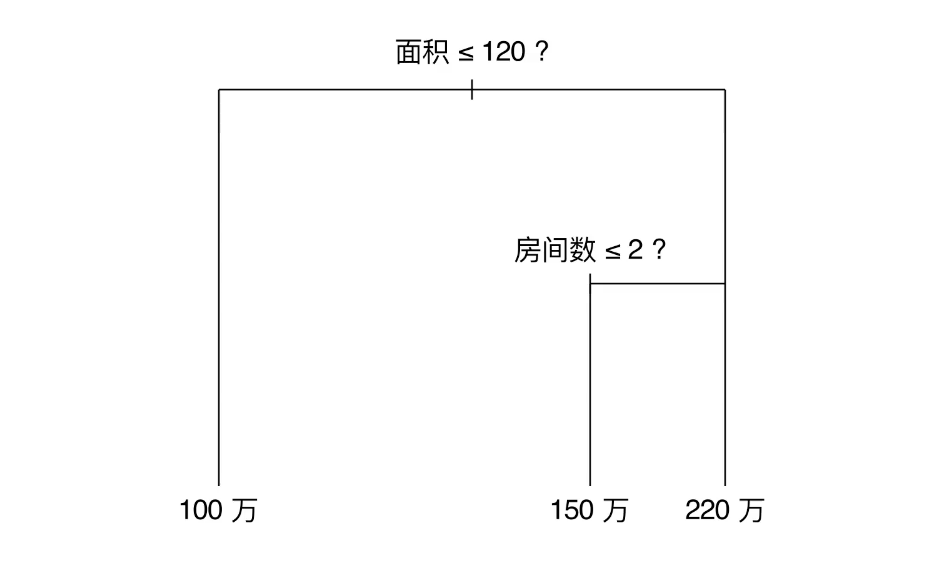
\includegraphics[width=0.5\linewidth,trim=0 0 0 0,clip]{image/regressiontree.png}
  \captionof{figure}{回归树的结构示意图：每个切分对应一个特征阈值，叶子节点给出预测值。}
  \label{fig:regression_tree}
\end{center}
这也就是为什么叫树。

\subsection{回归树的具体计算}
遗憾的是，
要想考虑将特征空间划分为 $J$ 个矩形区域的所有可能性，在计算上是不可行的。
因此一般采用一种 \textbf{自上而下} (top-down) 的 \textbf{贪婪} (greedy) 方法：
\textbf{递归二叉分裂} (recursive binary splitting)。
\begin{definition}[递归二叉分裂]
递归二叉分裂（Recursive Binary Splitting）是一种用于构建回归树和分类树的贪婪算法。其基本思想是：

\begin{enumerate}
  \item 从整个特征空间（即所有训练样本的集合）出发，选择一个特征 $X_j$ 及其切分点 $s$；
  \item 将样本划分为两个矩形区域：
  \[
    R_1(j,s) = \{ x \mid x_j \leq s \}, 
    \qquad
    R_2(j,s) = \{ x \mid x_j > s \} ;
  \]
  \item 选择使得残差平方和（RSS）最小化的分裂：
  \[
    \min_{j,s}\Bigg\{
      \sum_{x_i \in R_1(j,s)} (y_i - \hat{y}_{R_1})^2 \;+\;
      \sum_{x_i \in R_2(j,s)} (y_i - \hat{y}_{R_2})^2
    \Bigg\} ,
  \]
  其中 $\hat{y}_{R_m}$ 表示区域 $R_m$ 内训练样本响应的均值。
  \item 在每个新生成的区域内，重复上述步骤，直到满足停止条件（如区域样本数过小或树的深度达到上限）。
\end{enumerate}

该方法称为“递归”，因为分裂过程会不断重复；称为“二叉”，因为每次分裂都将一个区域划分为两个子区域；称为“贪婪”，因为每次分裂只考虑当前最优，而不是全局最优。
\end{definition}
\begin{dxtips}[贪婪算法-递归二叉分裂]
贪婪算法（Greedy Algorithm）：在每一步选择中，都作出在当前看来最优的局部选择，
而不从整体上进行考虑。
`自上而下'' 指的是从树的顶端（在此处，所有观测值都属于同一个空间）。
开始依次分裂预测变量空间，每个分裂点都会产生两个新的分支。
``贪婪'' 意味着在建立树的每一步中，\textbf{最优} (best) 分裂的确定仅限于这一步进程，
而不是针对全局去选择那些能够在未来过程中构建出更好树的分裂点。
二叉分裂法就是一旦他分割了一次，以后的分割都是在分割好的区域继续分割，不会从两个区域里面个拿出一部分产生一个新的区域即使这样会更好。
\end{dxtips}
\begin{proposition}[防止过拟合想要全局最优]
    上述方法会在训练集中取得良好的预测效果，却很有可能造成数据的过拟合，
导致在测试集上效果不佳。原因在于这种方法产生的树可能过于复杂。
一个分裂点更少、规模更小（区域 $R_1, R_2, \dots, R_J$ 的个数更少）的树
会有更小的方差和更好的可解释性（以增加微小偏差为代价）。

针对上述问题，一种可能的解决办法是：
仅当分裂使残差平方和 RSS 的减小量超过某阈值时，才分裂树节点。
这种策略能生成较小的树，但可能产生短视的问题：
一些起初看起来不值得的分裂在后面可能产生非常好的分裂，
也就是说，在下一步中，RSS 大幅减小。

因此，更好的策略是生成一个很大的树 $T_0$，
然后通过 \textbf{剪枝} (prune) 得到 \textbf{子树} (sub-tree)。
\end{proposition}
\begin{definition}[代价复杂性剪枝]
代价复杂性剪枝（Cost Complexity Pruning，又称最弱链接剪枝 weakest link pruning）
是一种用于从原始大树 $T_0$ 中选择最优子树的策略。该方法不是考虑所有可能的子树，
而是通过引入调整参数 $\alpha \geq 0$，在子树的复杂性和训练误差之间进行权衡。

对于给定的子树 $T$，其代价复杂度定义为：
\[
C_\alpha(T) = \sum_{m=1}^{|T|} \sum_{i: x_i \in R_m} (y_i - \hat{y}_{R_m})^2 \;+\; \alpha |T| ,
\]
其中 $|T|$ 表示子树 $T$ 的终端节点数，$R_m$ 表示第 $m$ 个终端节点对应的区域，
$\hat{y}_{R_m}$ 是区域 $R_m$ 内训练集的平均响应值。

当 $\alpha = 0$ 时，$C_\alpha(T)$ 仅度量训练误差，最优子树为原始大树 $T_0$；
随着 $\alpha$ 增大，终端节点数较多的子树将因复杂性受到惩罚，
使得更小的子树可能成为 $C_\alpha(T)$ 的最优解。
因此，通过调节 $\alpha$ 并最小化 $C_\alpha(T)$，
我们可以在模型复杂度和泛化能力之间找到平衡，从而选出合适的子树。
\end{definition}
也就是最开始的大树太复杂了想砍掉一些枝桠，但是砍的太多就预测的太不准了，砍完枝桠的RSS就是$C_{\alpha}$前面的部分。为了鼓励结构尽可能简单，后面加入T复杂度的权重，权重值为$\alpha$。权重值越高说明越倾向简答的结构。
\begin{dxtips}
    这是一种二次优化的思想，每当想引入新的维度的指标的时候都可以加入带权重的数。这正是 正则化 / 多目标优化 的思想。
\end{dxtips}

\begin{example}[算法 8.1 建立回归树]
\begin{enumerate}
  \item 利用递归二叉分裂在训练集中生成一个大树，只有当终端节点包含的观测值个数低于某个最小值时才停止。
  \item 对大树进行代价复杂性剪枝，得到一系列最优子树，子树是 $\alpha$ 的函数。
  \item 利用 $K$ 折交叉验证选择 $\alpha$。具体做法是将训练集分为 $K$ 折。对所有 $k=1,2,\dots,K$，有：
  \begin{enumerate}
    \item[(a)] 对训练集上所有不属于第 $k$ 折的数据重复步骤 1 和步骤 2，得到与 $\alpha$ 一一对应的子树。
    \item[(b)] 求出上述子树在第 $k$ 折上的均方预测误差。
  \end{enumerate}
  上述操作结束后，每个 $\alpha$ 会有相应的 $K$ 个均方预测误差，对这 $K$ 个值求平均，选出使平均误差最小的 $\alpha$。
  \item 找出选定的 $\alpha$ 值在步骤 2 中对应的子树即可。
\end{enumerate}
\end{example}
\begin{definition}[分类树]
    分类树（classification tree）和回归树十分相似，它们的区别在于：
分类树被用于预测定性变量而非定量变量。也就是研究是什么，而不是是多少的问题。在回归树中，
对一给定观测值，响应预测值取它所属的终端节点内训练集的平均响应值。
与之相对，对分类树来说，给定观测值被预测为它所属区域内的训练集中
最\textbf{常出现的类} (most commonly occurring class)。

\end{definition}
分类树的构造过程和回归树也很像。与回归树一样，分类树采用递归二叉分裂。
但在分类树中，RSS 无法作为确定二叉分裂点的准则。
一个很自然的替代指标是\textbf{分类错误率} (classification error rate)。
既然要将给定区域内的观测值都分到此区域的训练集上最常出现的类中，
那么分类错误率的定义为：此区域的训练集中非最常见类所占的比例。
其表达式如下：
\[
E = 1 - \max_k \big(\hat{p}_{mk}\big),
\tag{8.5}
\]
上式中的 $\hat{p}_{mk}$ 表示第 $m$ 个区域的训练集中的第 $k$ 类所占比例。
但事实上，分类错误率这一指标在构建树时不够敏感。
在实践中，另外两个指标更有优势。
\begin{definition}[基尼系数]
基尼系数（Gini index）用于度量分类树节点的纯度，其定义为
\[
G = \sum_{k=1}^K \hat{p}_{mk} \,(1 - \hat{p}_{mk}),
\tag{8.6}
\]
其中，$\hat{p}_{mk}$ 表示第 $m$ 个区域的训练集中第 $k$ 类所占的比例。

基尼系数可以理解为 $K$ 个类别的总方差。如果所有 $\hat{p}_{mk}$ 的取值都接近于 $0$ 或 $1$，
则基尼系数会很小。因而，基尼系数常被视为度量节点\textbf{纯度} (purity) 的指标：
若基尼系数较小，就意味着该节点包含的观测值几乎都来自同一类。也是Bernoulli 方差 
\end{definition}
\begin{itemize}
  \item $p$ 表示某个类别的占比；
  \item $1-p$ 表示“其他类别的占比”；
  \item $p(1-p)$ 则反映了一个类与其他类的对立程度：
    当分布均衡时（$p$ 和 $1-p$ 接近），该值最大；
    当一边占绝对优势时，该值趋近于 $0$。
\end{itemize}
熵（Entropy）也可以用来替代基尼系数作为分类树分裂指标，其定义为
\[
D = - \sum_{k=1}^K \hat{p}_{mk} \log \hat{p}_{mk},
\tag{8.7}
\]
其中，$\hat{p}_{mk}$ 表示第 $m$ 个区域的训练集中第 $k$ 类所占的比例。

由于 $0 \leq \hat{p}_{mk} \leq 1$，可知 $0 \leq - \hat{p}_{mk}\log \hat{p}_{mk}$。
显然，如果所有 $\hat{p}_{mk}$ 的取值都接近于 $0$ 或 $1$，则熵值接近于 $0$。
因此，与基尼系数类似，如果一个节点的纯度较高，则熵值较小。
事实上，基尼系数和熵在数值上是相当接近的。

在建立分类树的过程中，无论基尼系数还是熵，通常都用于度量某个分裂点的分类质量。
与分类错误率相比，这两种方法对节点纯度更敏感。
上述三种方法都可以用于树的剪枝，但若希望追求较高的预测准确性，最好选择分类错误率。
\section{装代法}
\begin{definition}[装袋法（Bagging）]
在一般情况下难以取得多个训练集，因此可以使用自助法（Bootstrap）作为替代，
即从某一个单一的训练集中重复取样，生成 $B$ 个不同的自助抽样训练集。
然后在第 $b$ 个自助抽样训练集上拟合模型并得到预测值 $\hat{f}^{*b}(x)$。
最后对所有预测值取平均，得到装袋法预测函数：
\[
\hat{f}_{\text{bag}}(x) = \frac{1}{B} \sum_{b=1}^B \hat{f}^{*b}(x).
\]
\end{definition}
决策树（Decision Tree）通常具有较高的方差（high variance），
这意味着如果将同一个训练集随机拆分成两部分，分别建立回归树，
结果可能会差别很大。相比之下，像线性回归这类“简单模型”通常方差较小，
在不同的数据集上结果差别不会太大。为了降低这种高方差，
统计学习里常用一种通用技巧，称为\textbf{自助法聚集}
（bootstrap aggregation），简称\textbf{bagging}。
具体做法是：从训练集里反复有放回地抽样（bootstrap），得到多个子集；
在每个子集上分别建立一个模型（如决策树）；最后把这些模型的预测结果
通过平均或投票的方式组合起来。这样可以显著降低模型的方差，提高泛化性能。
装袋法可以显著改善回归模型的预测效果，尤其对决策树十分有效。
具体做法是：利用 $B$ 个自助抽样训练集分别构造 $B$ 棵回归树，
再对其预测结果取平均。这些树通常根深叶茂且未剪枝，每棵树方差高但偏差小，
通过平均可有效降低方差。事实证明，成百上千棵树的组合能大幅提升预测精度。

在分类问题中，装袋法同样适用。对于一个给定测试样本，记录 $B$ 棵树的预测类别，
再采用\textbf{多数投票}（majority vote），即将出现频率最高的类别作为整体预测结果。
\begin{definition}{袋外误差估计}
装袋法可通过袋外（out-of-bag, OOB）样本直接估计测试误差，而无需交叉验证。
在自助抽样中，每棵树约使用训练样本的三分之二，剩余三分之一即为该树的 OOB 样本。
对某个观测值，可用未包含它的约 $B/3$ 棵树进行预测，并将结果求平均（回归）
或多数投票（分类），得到该观测值的 OOB 预测。综合所有样本即可计算 OOB 均方误差
或分类误差，从而得到装袋法测试误差的有效估计。事实证明，当 $B$ 足够大时，
OOB 误差与留一法交叉验证误差近似等价。
\end{definition}
即使装袋法树的集合比单个树解释数据要困难得多，
也可以用 RSS（针对装袋法回归树）或基尼系数（针对装袋法分类树），
对各预测变量的重要性做出整体概括。
\section{随机森林}
\begin{definition}[随机森林]
    随机森林（random forest）通过对树做去相关处理，实现了对装袋法树的改进。
在随机森林中，需要对自助抽样训练集建立一系列决策树，这与装袋法类似。
不过，在建立这些决策树时，每个分裂点不再考虑全部的 $p$ 个预测变量，
而是从中随机抽取 $m$ 个预测变量作为候选。该分裂点所用的预测变量只能从
这 $m$ 个候选变量中选择。在每个分裂点处都要重新抽取 $m$ 个预测变量，
通常 $m \approx \sqrt{p}$。也就是说，每个分裂点所考虑的预测变量个数约等于
总预测变量数的平方根。例如，在 Heart 数据集中共有 $13$ 个预测变量，
则取 $m=4$。
\end{definition}
这个目的就为了防止用装袋法生成的树都长的太相似。比如说都会选择最重要的变量作为顶部分裂点。问题是，与对不相关的量求平均相比，对许多高度相关的量求平均带来的方差减小程度
是无法与前者相提并论的。具体而言，在这种情况下，这意味着装袋法与单个树相比
不会带来方差的明显降低。
但是随机森林因为是随机取出m个预测变量作为候选，那么最强的变量可能都不在里面，这样的话次强变量等等都可能作为顶部分裂点等塑造出不一样的树。
\begin{itemize}
  \item 10 个人都参考同一个答案抄作业 $\;\Rightarrow\;$ 他们错的地方一样，平均结果还是错的。
  \item 10 个人各自独立思考 $\;\Rightarrow\;$ 有人错有人对，平均结果更接近真值。
\end{itemize}
分类聚类然后神经网络把深度学习结合到Matlab上边做边学
\end{document}